\documentclass[11pt]{book}

\usepackage{comment}
\usepackage{times}
\usepackage{natbib}
\usepackage{fullpage}
\usepackage{moreverb}
\usepackage{amsmath}
\usepackage{lscape}

\bibliographystyle{plain} % prsty, unsrt
%\usepackage[gather]{chapterbib}
\usepackage{bibunits}

\usepackage{hyperref}
\input{WebMacros}
\input{Smacros}
\input{XMLMacros}
\input{HTMLMacros}

\def\lt{$<$}
\def\gt{$>$}


\usepackage[pdftex]{graphicx}

\def\env#1{\texttt{#1}}
\def\Rfunc#1{\textbf{\texttt{#1()}}}
\def\Rcode#1{\texttt{#1}}

\begin{document}

\tableofcontents
\pagebreak

\subsection*{Preface} 
\addcontentsline{toc}{subsection}{Preface}

The aim of this book is to provide a text for both upper-division
undergraduates and graduate students in the area of statistical and
scientific computing with data.  The emphasis is on both the
high-level concepts and practical idioms of programming languages for
scientific computing, and both data and Web technologies, and
visualization that are increasingly important in the practice of
science.  We are in a remarkable era where data for so many
interesting and important problems are immediately available via the
Web to anyone who is interested.  To make use of it, however, we need
to have a modern vocabulary and set of skills to be able to access and
manipulate such data.  These skills are novel for statisticians as
they are rarely part of the curricula for either undergraduates or
graduates.  For the good of our field and science generally, however,
this has to change. We hope this book will prove to be useful in this
modernization of both the statistics curricula and also the way and
spirit at which statisticians view their discipline as transforming
into data and information science.


Originally, this book was aimed at upper-division undergraduates.  The
intent was to teach them the basics of statistical computing so that
they would be able to access, explore and present real data in the
context of meaningful investigations.  We wanted them to be able to be
productive and engaged in analyzing data and exploring statistical
methodology via simulation.  We hoped that the material would both
provide a strong foundation in being able to work with data, but also
teach them how to learn about new technologies in this fast changing
environment.

We subsequently decided to grow the book to contain additional, less
fundamental but important topics for more advanced students. The aim
was to address Master's students interested in more advanced
computational topics. This subsequently grew into additional topics
that are of interest to PhD students also and on into new technologies that
we envisage becoming increasingly relevant and popular for
statisticians (e.g. visualization with Google Earth, Web based
interactive graphics and composition, inter-system interfaces).  Some
of this material is recent research but very relevant and practical
for the practice of statistics.

We believe that the book will also be of interest to students and
practitioners in other fields.  We cover many fundamental tools of
scientific computing and programming generally.  These include core
tools that are hidden from casual users but which are important to
understand generally as one becomes more sophisticated.  These include
advanced topics such as the UNIX shell, make, linking and loading
compiled code, etc., but also new paradigms for data visualization
using Web technologies and data acquisition.

There are several books that cover many of the topics we
cover. However, there are very few books that cover all, or even a
significant subset of, the topics we present. Secondly, many books
that cover these topics act as relatively brief introductions or
references.  In this book, we have strived to present not only the
technical details and the how-to of the technologies, but also discuss
how to think about them, when to use them, compare different idioms,
paradigms and approaches.  Generally, we try to engage the reader in
thinking about the material and why it was designed that way, what
alternatives might be, and to be able to think about it rather than
simply mimic and connect lines of code.  The hope is that the reader
will have a deeper understanding and an ability to reason about
problems and approaches because of this understanding.  This is an
ambitious goal and may not be the aim of all readers.  However, we do
think that it is important for more statisticians and scientists
generally to become much more expressive computationally and this
requires not just learning the vocabulary, but style and presentation.
Other books very understandbly focus on 

This book is intended to be a textbook but also a guide for
practitioners.  We do not expect that an instructor would teach more
than half of the material in any course.  We do think however it is
useful to illustrate to students that there is more to scientific and
statistical computing than any of basic programming, simple
visualization, data technologies, Web services, advanced computing
techniques, algorithms and computational statistical methods.  We
expect that a curious student might read this book by herself to learn
important foundational material that we would like our good students
to know so that they can be complete statisticians who can exploit the
power of computing to do good data analysis and statistical research.







\chapter{Introduction}

\chapter{Introduction to Programming:  Getting Started}

\chapter{The Foundations of the Language}

%\documentclass{article}
\def\SFunction#1{\textbf{#1()}}
\def\SArg#1{\textsl{#1()}}
\usepackage{times}
\usepackage{fullpage}
%\def\long\question#1{\textit{#1}}
\def\question#1{\textit{#1}}
\usepackage{graphicx}
\usepackage{amsmath}
\author{Duncan Temple Lang}
\title{Approaches for Random Number Generation}
\begin{document}
\maketitle

Statistics attempts to make sense of randomness.  It also uses
randomness in a variety of different ways to perform computations.
Cross-validation involves random permutations of the observations to
create the K-fold test sets.  Similarly, the non-parametric bootstrap
involves sampling with replacement from the observational units.  And
the parametric bootstrap involves sampling from probability
distributions.  R, S-Plus, Matlab and other commonly used software
environments provide functions for for generating random variates from
common probability distributions.  And one is well advised to use
these when they exist as they are likely to be more efficient and
better tested than code that we create ourselves as part of a bigger
project.  In spite of the availability of these common distributions,
we often encounter situations where we need to generate values from a
distribution that is not built-in to these environments.  Generally,
there are several approaches to go about creating samples from these
less common distributions.  One is called the Inverse CDF method.
Another is Acceptance/Rejection sampling.  And a third is Markov Chain
Monte Carlo.

Underlying the computations of all these methods is the ability to
generate pseudo random numbers on a computer. For that we need
suitable random number generators.



\section{Inverse CDF Method}

Suppose we have a random variable $X$ with density function $f_X(x)$
and we want to generate sample values from the corresponding random
variable.  If we can get the inverse function ($F_X^{-1}(x)$) of the
CDF of $X$, then we create a new random variable using the following very
simple procedure:
\begin{itemize}
\item generate a sample, $u$,  from a $U(0, 1)$, i.e. a
 standard Uniform distribution
\item compute $y = F_X^{-1}(u)$.
\end{itemize}
The value $y$ is clearly random since it is based on a random input,
$u$.  And we have a random variable $Y$ defined by this random
procedure.  It turns out that its density is $f_X(x)$, exactly what we
want to sample from. So this procedure generates values from the
random variable $X$ as we set out to do.


It is reasonably easy to verify that the density of our random
variable $Y = F^{-1}(U)$ (where $U ~ U(0,1 )$) is $f_X(x)$, or
equivalently and more readily that the CDF of $Y$ is $F_X(x)$.
\begin{eqnarray*}
 Pr(Y \le x)  &=& Pr(F_X^{-1}(U) < x) \\
  &=& Pr(F_X(F_X^{-1}(U)) < F_X(x)) \\
  &=& Pr(U < F_X(x)) \\
  &=& F_X(x)
\end{eqnarray*}
We use the fact that $F_X$ is monotonically non-increasing and has an
inverse in the step that moves from $Pr(F_X^{-1}(U) < x)$ to the
equivalent $Pr(F_X(F_X^{-1}(U)) < F_X(x))$.  
Also the CDF of a standard uniform is  $F(u) = u$
which follows from integrating the density $f_U(u) = 1$ between
$0$ and $1$.
And the result is simply
that $Y$ has a CDF $F_X(x)$ which is what we wanted to show.

A simpler or more intuitive way to think about why $Y$ has the CDF
$F_X(x)$ is the following.  What we are doing is sampling a percentile
at random when we pick a number $u$ between $0$ and $1$, or $0$ and
$100\%$.
Then we are asking for the corresponding quantile of
the $X$ distribution, i.e. the value $x_u$ of the random
 variable $X$ such that 
 $$F_X( x_u) = u$$ This is easily obtained by using the inverse of
 $F_X$.  So we are matching quantiles of the $U(0, 1)$ distribution
 with the corresponding value in $F_X(x)$.  And by randomly sampling
 the quantiles in $U(0, 1)$, we get random samples from $F_X(x)$.


Since we have the computer at our fingertips, we can verify that the
resulting density is what we expect.  Let's consider a very simple
case, the Exponential distribution.
One parameterization of the density of an Exponential distribution is given as
$$ f_E(x, \lambda) = \frac{1}{\lambda}e^{-x/\lambda}$$ where $\lambda
> 0$ and $x \in (0, \infty)$.
Simple integration gives us the CDF as
$$ F_E(x, \lambda) = 1 - e^{-x/\lambda}$$
The inverse of this function is easy to get.
Let $R$ be $F_E(x, \lambda)$.
Then 
\begin{eqnarray*}
  R &=& 1 - e^{-x/\lambda} \\
  1-R &=& e^{-x/\lambda} \\
  \log(1 - R) &=& -x/\lambda \\
  x &=&  -\lambda \log(1 - R)
\end{eqnarray*}
So 
$$ F^-1_E(x, \lambda) = -\lambda \log(1 - x)$$


% Since we are going to evaluate this at values from a random Uniform,
% we can replace $\log(1 - x)$ with $-\log(x)$ since if $x ~ U(0, 1)$,
% then so is $1 - x ~ U(0, 1)$.

R uses the other parameterization for an Exponential density,
namely
$$ f_E(x) = \alpha e^{- x \alpha}$$ In other words, $\alpha =
1/\lambda$ in the earlier parameterization.  Remembering this, we can
generate a random sample using both the Inverse CDF method and also
from R's built-in \SFunction{rexp} generator.
We will use $\lambda = 4$ and hence $\alpha = .25$.
\begin{verbatim}
u = runif(10000)
x.e = - 4 * log(1 - u)
hist(x.e, prob = TRUE, xlab="X", 
     main = expression(paste("Exponential Distribution: ", lambda == 4)))
curve(dexp(x, .25), 0, max(x.e), add=TRUE, col = "red")
\end{verbatim}

\begin{figure}[htbp]
  \begin{center}
    \leavevmode
     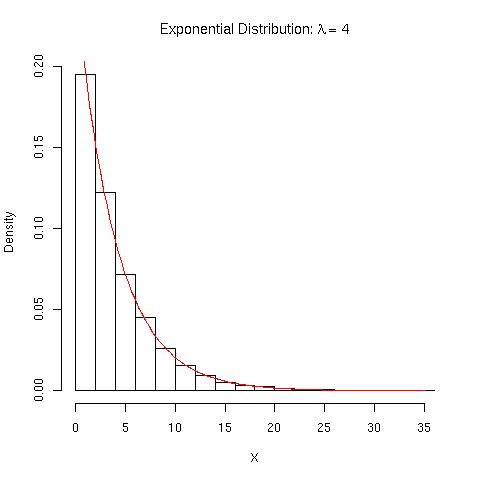
\includegraphics{expInv.jpg}    
    \caption{Sample from an Exponential(4)}
    \label{fig:expInv}
  \end{center}
\end{figure}


We can compare moments of the sample with what we expect.
\begin{verbatim}
> c(mean(x.e), var(x.e))
[1]  3.970798 15.611575
> x.s = rexp(10000, .25)
\end{verbatim}
And we can generate a sample from 
R's built-in generator and compare
the moments.
\begin{verbatim}
> c(mean(x.s), var(x.s))
[1]  3.959364 15.889116
\end{verbatim}
And these agree up to sampling error
with the values $4$ and $16$.

Of course, this simulation does not prove that the inverse CDF method
gives us a random variable with CDF $F_X(x)$.  We needed the math for
that. However, the computer does allow us to explore the technique and
get an understanding of it for particular distributions.

We use the Exponential distribution to illustrate the basics of the
Inverse CDF method. But of course we had the built-in generator
available in R so there was no need.  And, indeed, the generation
technique in R uses a different approach (given by Ahrens and Dieter).
One reason for avoiding the Inverse CDF method is that computing
$F^-1_X(u)$ may be computationally expensive relative to another
approach.  However, the Inverse CDF method is useful when the CDF is
invertible and that inverse function has a reasonably simple form and
there are no built-in functions available to us!  For example, let's
consider a random variable whose distribution is given by the
triangular distribution.  This has a density given
$$
  f_X(x) = 
  \begin{cases}%
   \frac{2(x - a)}{(b-a)(c-a)} & 0 \le x < c, \\
   \frac{2(b -x)}{(b-a)(b-c)} & c \le x \le b \\
   0 & x \not\in [a, b]    
  \end{cases}
$$
and is shown in figure \ref{fig:triangularDensity}.
\begin{figure}[htbp]
  \begin{center}
    \leavevmode
    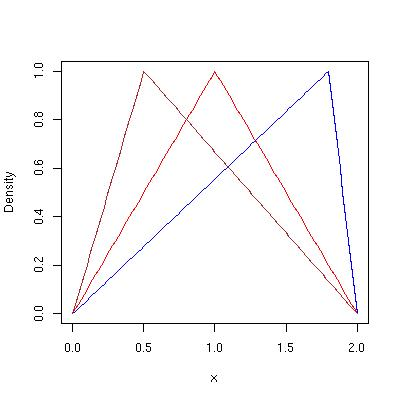
\includegraphics{triangularDensity.jpg}
    \caption{The Triangular Distribution Density.
   These are three different triangular distributions
   on the  interval $[0, 2]$
    with parameters
    $(0, 2, .5)$ (brown), $(0, 2, 1)$ (red), and $(0, 2, 1.8)$ (blue).
   }
    \label{fig:triangularDensity}
  \end{center}
\end{figure}
One can determine these formulae using
the fact that since this is a density, it 
must integrate to $1$. Since we have two triangles
and the area of a triangle is 
$1/2$ base $\times$ height, we get
\begin{eqnarray*}
 1 & = & 1/2 (c-a)\times h + 1/2 (b-c) \times h \\
 2 &=& (b-a) \times h \\
 h &=& 2/(b-a)
\end{eqnarray*}
Then, we have the two points on each line
and we can use the formula for a line.


We can integrate the two components
in the density to get the CDF.
This yields
$$
  F_X(x) = 
  \begin{cases}
  \frac{(x - a)^2}{(b-a)(c-a)} & 0 \le x < c\\
                  1 - \frac{(b -x)^2}{(b-a)(b-c)} & c \le x \le b \\
                  0 & x < 0 \\
                  1 & x > b
  \end{cases}
$$

And finally, we must compute the inverse.  Unlike the case of the
exponential distribution, we have a quadratic function here and we
have two roots.
Taking the case where $c \le x < b$, we have
\begin{eqnarray*}
  R = 1 - \frac{(b-x)^2}{(b-a)(b-c)} \\
  (1 - R)(b-a)(b-c) = (b-x)^2 \\
  \sqrt{(1 - R)(b-a)(b-c)} = b - x \\
\end{eqnarray*}
We can ignore the other root which is $-\sqrt{(1 - R)(b-a)(b-c)}$
because $b - x$ must be positive as $x \le b$ and also $R < 1$ since
it is our uniform random number.  We can similarly invert the other
term in the CDF.  All that is left is that we need to determine the
intervals for which these two pieces in the inverse CDF apply.  The
splitting point on the X axis is $c$.  However, we need this on the
uniform - $[0,1]$ - scale.  The breakpoint on this scale is the
probability or area under the CDF up to the point $c$.
In other words, it is the area of the left triangle in 
the distribution. And this is
$1/2 (c-a) h$  = $(c-a)/(b-a)$. So the 
inverse of the CDF is 
$$
  F^{-1}_X(x) =
  \begin{cases}
    \sqrt{x(b-a)(c-a)} + a &  0 \le x < (c-a)/(b-a)\\
    b - \sqrt{(1 - x)(b-a)(b-c)} & (c-a)/(b-a) \le x \le 1 \\
    0 & x < 0 \\
    1 & x > b
  \end{cases}
$$

And now we can generate random numbers from a Triangular
distribution with parameters $(a, b, c)$ with $(a \le c \le b)$
using the R function
\begin{verbatim}
rtriang =
function(n, a = 0, b = 2, c = 1) {

    if(!(a <= c && c <= b))
      stop("Incorrect parameters")

    x = runif(n)

    ans = rep(0, length(x))
    ans[x > b] = NA

    cutPoint = (c-a)/(b-a)
    A = (x > a & x < cutPoint)
    B = (x >= cutPoint & x <= b)

    ans[A] = sqrt(x[A]*(b-a)*(c-a)) + a
    ans[B] = b - sqrt((1-x[B])*(b-a)*(b-c)) 

    ans
}
\end{verbatim}

Now we can generate our samples and compare the
result
\begin{verbatim}
x = rtriang(10000, 0, 3, 1)
hist(x, prob = TRUE, xlab= "X", main = "Triangular(0, 3, 1)")
curve(dtriang(x, 0, 3, 1), 0, 3, add = TRUE, col = "red")
\end{verbatim}
And, of course,  we get very good agreement with 
the only difference being sampling variability.


\subsection{Distributions}
There are several common distributions that are amenable to the
Inverse CDF method.  We have seen the triangular and exponential
distributions.  The Extreme value, geometric, logistic, Pareto and
Weibull distributions can also be handled in this way.
The Extreme value distribution has density and CDF given
by
\begin{eqnarray*}
f_{\hbox{Extreme Value}}(x) &=& \frac{1}{\beta}e^\frac{x-\mu}{\beta}e^{-e^{\frac{x-\mu}{\beta}}} \\
F_{\hbox{Extreme Value}}(x) &=& 1 - e^{e^\frac{x - \mu}{\beta}}  
\end{eqnarray*}

The CDF of the Geometric is
\begin{equation}
  F_{\hbox{Geo}}(x) = 1 - (1-p)^x
\end{equation}


The CDF of the Logistic is
\begin{equation}
  F_{\hbox{Logistic}}(x) = 1 - 1/(1 + e^{(x - \mu)/b})
\end{equation}

The CDF of the Pareto is
\begin{equation}
  F_{\hbox{Pareto}}(x) = 1 - x^a
\end{equation}

And the CDF of the Weibull is
\begin{equation}
  F_{\hbox{Weibull}}(x) = 1 - e^{(x/a)^b}
\end{equation}



\section{Rejection/Acceptance Sampling}
The Inverse CDF approach works well if a) we can obtain a formula for
the inverse CDF, b) evaluating the formula for a given $u$ is not
excessively expensive.  If we have a density function $f_X(x)$ and we
cannot get the inverse of its CDF, then we are stuck.  How can we
generate random values from that density?  Jon Von Neumann, the
``father of computer architecture'', devised a procedure that allows
us to create samples from essentially arbitrary density functions,
$f_X(x)$.  The idea is quite simple and intuitive.  Let's focus on a
particular density, say the $\beta(4, 3)$.  This is
shown in figure \ref{fig:beta43}.
\begin{figure}[htbp]
  \begin{center}
    \leavevmode
    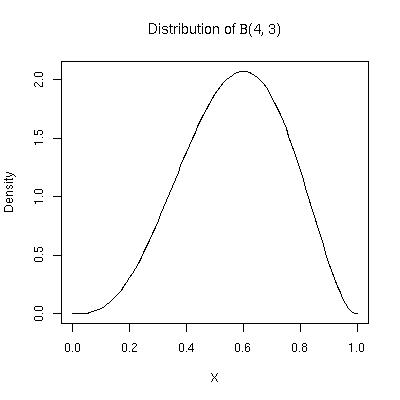
\includegraphics{beta43.jpg}
    \caption{Beta distribution - $\beta(4, 3)$}
    \label{fig:beta43}
  \end{center}
\end{figure}
What we really want to do is sample uniformly from the region under
this density.  If we could throw an infinite number of darts at the
2-dimensional plane $\Re \times \Re$ in a random way, then we could
consider only the darts that were within the region described by the
density.  Then we could take the $X$ coordinate of each of those darts
and that would constitute a random sample.  And these values would
have the appropriate density $f_X(x)$.  You should convince yourselves
that they do have the desired density.

Now, there are two problems with this approach.  We have to throw a
lot of darts!  This is time consuming and perhaps dangerous.  And if
we really throw them at random onto the entire plane, we will waste an
enormous amount of them.  Specifically, a relatively small proportion
will actually end up under the density.  After all, we are only
looking for values under the curve that ranges from $0$ to $1$ on the
X axis and from $0$ to $2.08$ on the Y axis. (\question{How can we
  determine this value?}).  What we are looking for is a more
efficient mechanism that we can use on a computer.

If we really could throw darts, we would try to narrow down the area
at which we are throwing them so that we wouldn't waste as many.
Suppose we consider the rectangle that encloses this entire density,
namely the Cartesian region $[0,1] \times [0, 2.08]$
shown in figure \ref{fig:beta43Unif}
\begin{figure}[htbp]
  \begin{center}
    \leavevmode
    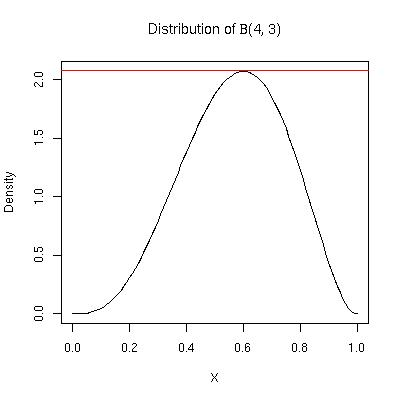
\includegraphics{beta43Unif.jpg}
    \caption{Envelope of the $\beta(4, 3)$ density.}
    \label{fig:beta43Unif}
  \end{center}
\end{figure}
If we could throw darts only in this region, then many more would be
actually ``accepted'' in our sample, i.e. be within the region under
the density.

This is the basic idea.  We try to sample uniformly from under the
density, but we cannot do this easily.  So we try to sample uniformly
from a bigger region that encloses the area of interest (our density)
and then we take only the samples within our area of interest.  If we
agree that this is a strategy that would yield a sample with the
correct distribution, i.e. with a density $f_X(x)$ then we have only
one thing left to figure out.  And that is how can we do this
practically and on a computer?

The answer involves a two-step random procedure.  We have to sample
the larger region that encloses our density.  Unlike our other random
number generation techniques, this involves sampling from a $2$
dimensional region.  So we want to avoid this if possible.  What we
will do is quite clever, thanks to John Von Neumann.  We break this
into two $1$ dimensional sampling steps.  What we do is to find a
random variable that we can sample from.  Ideally, it would have the
same \textit{support} (i.e. range) as the random variable of actual
interest (i.e the on with density $f_X(x)$).  Then, we generate a
second value that gives us the second dimension.  And this allows us
to sample uniformly in the larger region. And then we do our
``rejection-acceptance'' trick by checking whether the point is inside
the region in which we are actually interested. 

We have described this procedure in words. At some point we have to
put this into technical terms so that we can use it on the computer.
And we will also need to write it mathematically so that we can prove
that the resulting random procedure creates random values with the
correct density.  So now is a good time.  Let's suppose we can find a
second probability density function, $g_Y(y)$ that we can sample from.
Obviously, this must integrate to $1$. So its area is the same as the
density in which we are interested, $f_X(x)$.  So we know that the
density $g_Y()$ cannot entirely contain $f_X(x)$.  However, what if we
could multiply this density $g_X(x)$ by some number $c$
so that 
$$ c \times g_Y(x) \ge f_X(x) \forall x.$$ If this is possible, then
we can do the following.  Generate a random value from the density
$g_Y()$, say $y$.  Then, generate a value ($u$) from a Uniform
distribution between $0$ and $c g_Y(y)$.  We accept $y$ as being a
value in our target sample if $u < f_X(y)$.
In other words, if $u$ is within the region enclosed by $f_X(x)$,
we keep it; otherwise we reject it and return to the original
sampling steps.

So the acceptance/rejection sampling procedure in more algorithmic
terms is as follows:
\begin{enumerate}
\item Select $g_Y(y)$ and $c$ such that  
    $c g_Y(x) > f(x) \forall x$ of interest.
\item Generate a random value, $y$,  from $g_Y()$.
\item Generate a random value, $u$, from $U(0, c g_Y(y))$.
\item Accept $y$ if $u \le f_X(y)$.
  Otherwise, return to step $2$.
\end{enumerate}


Let's return to our example of the $\beta(4, 3)$.  One of the simplest
choices for $g_Y()$ is the uniform distribution.  It is especially
simple in this case as the $\beta(\cdot, \cdot)$ distribution has
support on the interval $[0, 1]$, just like $U(0, 1)$.  We then need
to select $c$ so that the density $c$ times the density $g_Y(y) = 1$
is greater than the density of the $\beta(4, 3)$.  We can eyeball this
by plotting the density $f_X(x)$ and taking a sufficiently large value
of $c$.  From figure \ref{fig:beta43Unif}, we see that anything above
$\approx 2.1$ is fine. So $2.5$ will work to be on the safe side.

What happens if we chose $c$ conservatively?  We are enlarging the
region in which we take our potential sample of values.  The larger
this is relative to the region under the density $f_X(x)$, the greater
the number of samples that will be rejected.  As a result, we will
have to generate more potential samples if we need to get a fixed
number $n$ accepted samples.  So choosing our enveloping region as
close as possible to the region of interest (i.e. under $f_X(x)$) is
highly desirable. When using the Uniform distribution, i.e. a
rectangular enveloping region, we want to chose $c$ to be the maximum
of our density $f_X(x)$.  A little calculus allows us to find this.
Alternatively, we can use R to obtain an approximate answer
by evaluating the density at different points 
\begin{verbatim}
 max(dbeta(seq(0, 1, length = 100000), 4, 3)
\end{verbatim}
yielding $2.07$.


So now we are set to perform the different steps to generate a value
from a $\beta(4, 3)$ random variable.
\begin{verbatim}
 while(TRUE) {
   y = runif(1)
   u = runif(1, max = 2.07 * y)
   if(u < dbeta(y, 4, 3))
     break
}
\end{verbatim}

I have written some functions that allow us to explore different
choices of $g_Y()$ and to generate samples.
Using a simple rectangular sampling region
via the standard Uniform density for $g_Y()$,
we get
\begin{figure}[htbp]
  \begin{center}
    \leavevmode
    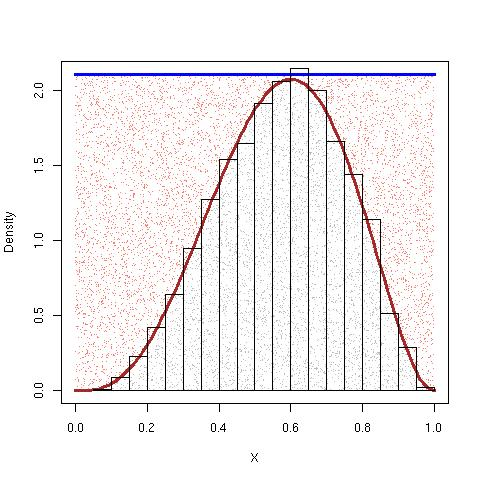
\includegraphics{ARSBetaUnif.jpg}
    \caption{Acceptance/Rejection using the triangular distribution}
    \label{fig:betaUnif.jpg}
  \end{center}
\end{figure}
The proportion of samples that were accepted is $47.3\%$.
We see that the sample histogram is very close to the
density and the variation is just sampling error.

By choosing a better enveloping region, we can improve the acceptance
rate.  In the case of the $\beta(4,3)$ density, we can use a
triangular distribution as $g_Y()$ and scale it to create an envelope
region. The particular choice of triangular distribution is $Tr(0, 1,
.8)$ and we choose $c$ to be $1.6$.  The plot in figure
\ref{fig:betaTriang.jpg} shows this region.
\begin{verbatim}
acc = ars.eg(function(x) dbeta(x, 4,3), 
             function(x) dtriang(x, 0, 1, .8), 
             1.6, 
             function(n) tr.inv(runif(n), 0, 1, .8), 
             10000)
\end{verbatim}
\begin{figure}[htbp]
  \begin{center}
    \leavevmode
    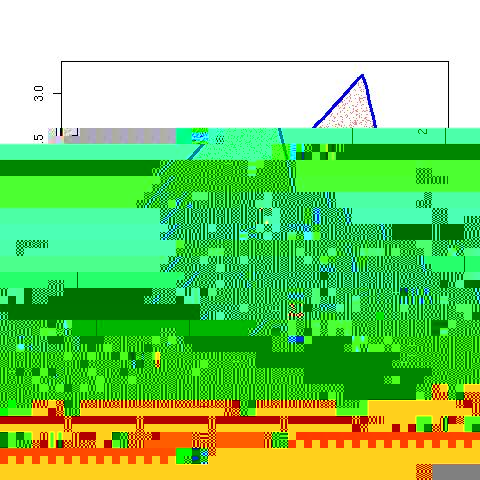
\includegraphics{ARSBetaTriangular.jpg}
    \caption{Acceptance/Rejection using the triangular distribution}
    \label{fig:betaTriang.jpg}
  \end{center}
\end{figure}
The acceptance rate for this is $62\%$.


\section{Markov Chain Monte Carlo - MCMC}
In most simulation contexts, we are interested in estimating the
expression $E_{f_X}[g(X)]$.
If we have i.i.d. samples from the random variable with density $f_X$
of the form $x_1, \ldots, x_n$, we can estimate this value
as
\begin{equation}\label{egx}
 E_{f_X}[g(X)] \approx \frac{1}{n} \Sigma_{i=1}^n g(x_i)
\end{equation}
The law of large numbers tells us that this is a good estimator.
Using different functions $g()$, we can obtain estimates for different
properties.  For example, $g(x) = x$ gives us the expectation of the
random variable.


Identical and independent values may be hard to sample from $f_X(x)$.
But we can use the estimator above in \ref{egx} if the $x_i$ are not
independent but sampled from $f_X(x)$ in proportion to $f_X()$.  The
computation of the variance is more complicated in these
circumstances, but the estimator is good.  This is because
\begin{equation}
  E_{f_X}[g(x)] = \int g(x) f_X(x) dx
\end{equation}
So if we can generate $x_i$ from $f_X()$ we can use Monte Carlo to
solve many problems.

The problem that we are now faced with is how to generate sample
values from the density $f_X(x)$, dependent or independent.  It turns
out that this is actually quite simple if we use what are called
Markov Chains.  Consider the following technique for generating a
sequence of random values.  Define $X_{t+1}$ by sampling from a
distribution that only depends on $X_t$, i.e. the current state of the
sequence.  In other words, we have a probability distribution given in
general terms as $P(X_{t+1} \vert X_t)$.  This sequence ${X_t}$ is
called a Markov chain.

To get the sequence started, we need a starting value $X_0$.  But
$X_{t}$ will depend on the value of $X_0$.  For many probability
distributions $P(X_{t+1} | X_t)$, it turns out that $P(. | X_0)$ is
independent of $X_0$ and it doesn't matter where we start.  And under
certain conditions, the sequence ${X_t}$ converges to a stationary
distribution, $\pi(x)$, which does not depend on $t$ or $X_0$.  Thus
for a sufficiently large value of $t$, $t_0$, $X_{t_{0} + 1}, X_{t_{0}
  + 2}, \ldots$ are samples (\textit{not} necessarily independent)
from the density $\pi(x)$.
So we can estimate $E_{g_X}[X]$ as 
\begin{equation}
  \frac{1}{n - t_0}\Sigma_{i = t_0}^n g(x_i)
\end{equation}


All that remains to use this technique is to create the Markov Chain.
In other words, we must specify the value $P(X_{t+1} \vert X_t)$ so
that we obtain the desired stationary distribution $f_X(x)$.  This
seems like a hard task, but it turns out to be quite simple.  Suppose
we have a distribution function $q(\cdot \vert X_t)$ which we will
call our \textit{proposal} distribution.  For a given $t$, we generate
a sample from a random variable $Y$ with this density.  We call $q()$
a proposal distribution because we don't use it directly to generate
$X_{t+1}$ in our sequence. Instead, we generate this new value but,
like acceptance/rejection sampling, we decide whether to accept it
under certain conditions.  Specifically, we use an decision algorithm
to accept or reject this new value.
The Hastings algorithm decides to accept this new value
with probability
$$
 min(1, \frac{f_X(Y)}{f_X(X_t)})
 $$ In other words, we toss a weighted coin with probability $ min(1,
 \frac{f_X(Y)}{f_X(X_t)})$ and if it turns up heads, we accept the new
 value $Y$ as the next step in the sequence, $X_{t+1}$.  If the coin
 ends up tails, we stay where we are and $X_{t+1} = X_t$.  This
 acceptance probability essentially favors $Y$ if $Y$ is more likely
 than the current value $X_{t}$.

The Metropolis-Hastings algorithm adds a variation to this.
Instead of looking at the likelihood ratio of $f_X(Y)/f_X(X_t)$,
it uses
$$
 \frac{q(X\vert Y) f_X(Y)}{q(Y\vert X) f_X(X)}
 $$ 
where $q$ is our proposal distribution again.
This yields nice properties that allow the Markov Chain to be
reversible and generally nicely behaved.

Regardless of which algorithm we use to accept or reject or our
proposal $Y$, the algorithm for generating the steps in the Markov
Chain are quite simple.

We need a function to generate a value from our proposal distribution.
This is the argument \SArg{r}.  To compute the acceptance probability,
we need $f_X()$, the stationary target density.  And if we are using
the Metropolis-Hastings algorithm we also need the density of the
proposal distribution given by \SArg{q}.  And we need a starting
point, $X_0$.  \SArg{n} says how many elements in the sequence we
should generate.  We need this to be large enough so that the chain
converges to $f_X()$ and yields sufficient sample values.
\begin{verbatim}
mcmc =
function(x.0 = 0, r, q, stationary, n = 1000, algorithm = metropolis)
{
     xs = numeric(n+1)  # space for the answers
     xs[1] = x.0
     for(i in 1:n) {
       y = r(xs[i])   # Generate proposal
       k = algorithm(xs[i], y, stationary, q)
       xs[i+1] = ifelse(runif(1) <= k, y, xs[i])
       if(is.na(xs[i+1])) {
        stop("Problems in MCMC")
       }
     }

     class(xs) <- "mcmc"
     xs
}
\end{verbatim}

Let's generate a sample from a t-distribution with $10$ degrees of
freedom, $t(10)$.  This is the stationary distribution that is our
target.  We can use the R function \SFunction{dt} to compute the
density.  We will use a Normal distribution as our proposal
distribution with mean $X_t$ and variance $1$.  We can use
\SFunction{rnorm} to generate proposal values and \SFunction{dnorm} to
calculate the density in the Hastings algorithm.
We'll generate $10,000$ values and then look at the last
$5000$ to give this adequate time to ``burn in'' or converge
to $t(10)$. We'll chose a strange starting value of $-10$
to illustrate how this converges.
\begin{verbatim}
 xt = mcmc(-10, 
           r = function(x) rnorm(1, x), 
           q = function(x, y) dnorm(y, x), 
           stationary = function(x) dt(x, 10), 
           alg = hastings, 
           n = 10000)
\end{verbatim}
We can see how well the sample approximates the
true density $t(10)$ in figure
\begin{figure}[htbp]
  \begin{center}
    \leavevmode
    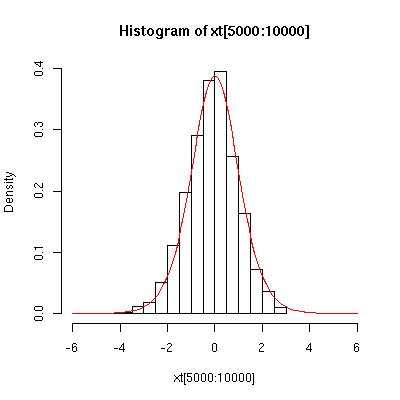
\includegraphics{mcmcT10.jpg}
    \caption{MCMC sample from $t(10)$.}
    \label{fig:mcmcT10.jpg}
  \end{center}
\end{figure}
This looks pretty close and within sampling variation.


The MCMC  approach to estimating $E[g(X)]$ and sampling dependent
values from a density is very powerful and is similar in ways to the
acceptance/rejection sampling we covered above.  One does have to
honor the conditions on the proposal and stationary distributions to
ensure that the Markov chain converges and converges to $f_X()$.


\end{document}



\chapter{Basics of Visualizing Data}
The basics of graphics devices, high-level plots,
annotating plots, and even 
\Rcode{par(mfrow = c(r, c))} and 
\Rfunc{layout}.

This will also  cover the basics of lattice.

\chapter{Data Input}
\section{Reading regular/tabular data.}
\section{More complex data}
\subsection{connections}
\section{Dealing with Large Data}

\chapter{Working with Complex Data: Text}


\chapter{UNIX Tools}
This chapter discusses the basics of using unix tools on different
platforms (Linux, Mac OS X, cygwin).  We present some of the standard
UNIX tools such as wc, grep, sort, uniq, cut, and so on.  We also
present the ideas of redirection and pipes and how we can connect the
output of one command as the input to another.  We also constrast
these approaches to using built-in R functions and how, under certain
circumstances, we can gain remarkably efficiency in our computations.
It also illustrates how we have to think about which tool we use for
particular tasks and how we can combine these tools for an overal
task. In this way, this is the initial introduction to inter-system
interfaces, but in a relatively traditional manner.


\section{The UNIX Command Line}
Thi chapter focuses on using the shell remotely or interactively
generally.  It builds on the previous chapter and may even be a
subsection.  This covers topics such job creation and control,
i.e. nohup, batch jobs, \&, kill.  We also cover ssh, scp, X11
forwarding, ssh configuration.

% Shells

%\input{Geolocation/Geolocation}

\chapter{Relational Databases}
%\def\SQLFunction#1{\textit{#1}}
\def\SQLName#1{\textsl{\Escape{#1}}}


%\begin{bibunit}
\chapter{Relational Database Management Systems}\label{chap:dbms}
 
%\Goal{Make it easier to read a DBMS book after reading this material
%and to understand how to use a database from within a statistical system
%and  when to understand when it is appropriate to use an RDBMS to
%manage data.
%}

\section{Introduction}

Databases are useful in many different scenarios.
For example, 
\begin{itemize}
\item Industry: Data collected from the manufacturing process are stored in
databases and those monitoring the production process need access to these
data as soon as they enter the database.  Also, those interested in improving
the quality of the product or increasing the yield need access to this data.

\item Clinical trial: Study how well a new drug or treatment works, and
in order for the Food and Drug Administration (FDA) to approve the drug
there must be convincing evidence that the treatment is safe and effective.
It is critical that accurate, reliable, and secure data are kept on
the patients involved.
These data are collected and reviewed by many different people, including:
doctors and nurses at multiple remote locations who monitor the health of the
patient, lab workers who process lab tests, social workers and
health care professionals who maintain contact with the patients,
and statistical analysts who study the effect of the treatment.

\item Retail: Information on inventory and sales for large retail
are stored in databases for up-to-date tracking of inventory and continual
monitoring of sales. 
Also market research groups ``mine'' for relationships to see if they 
can improve the supply chain network, design new marketing strategies, etc.
\end{itemize}

These examples give us many reasons whey we use databases.
In particular, databases:
\begin{itemize}
  \item Include meta-data, so the data are self-describing for any
  application 
  accessing them;
  \item coordinate synchronized access to data so users take turns
  updating information rather than overwriting each other's inputs;
  \item support client-server computing where the data are stored centrally
  on the server and clients at remote sites can access it;
  \item propagate information and enforce standards when updates, deletions,
        and additions are made;
   \item control access to the data, e.g. some users may have read-only access
   to a subset of the data while others may change and update information
   in the table;
   \item centralize data for backups;
   \item change continually and give immediate access to live data. 
\end{itemize}

Sometimes we do not need these functionalities to do our own work, but
others involved with the data do need them and so databases are 
imposed on us because of the corporate or institutional approach to
gathering and managing data.

\section{The Basic Relational Component: The Table}

The basic conceptual unit in a relational database is the two-dimensional table.
A simple example appears in Figure \ref{dbms:fig:CTsimple}, where the
table contains laboratory results and test dates for three 
patients in a hypothetical clinical trial. 
The data form a rectangular arrangement of values similar to a data frame,
where a row represents a case, record, or experimental unit,
and a column represents a variable, characteristic, or attribute of the cases.
In this example, the three columns correspond to a patient identification
number, the date of the patient's lab test, and the result of the test,
and each of the eight rows a specific lab test for a particular patient.
We see that patient \#101 received tests on four occasions, patient \#102 was 
given three tests, and the third patient has been tested only once.


\begin{figure}
\begin{tabular}{lll}
ID & Test Date & Lab Results \\
\hline
101 & 2000-01-20 & 3.7 \\
101 & 2000-03-15 & NULL \\
101 & 2000-09-21 & 10.1 \\
101 & 2001-09-01 & 12.9 \\
102 & 2000-10-20 & 6.5  \\
102 & 2000-12-07 & 7.3  \\
102 & 2001-03-13 & 12.2 \\
103 & 2000-02-16 & 10.1 \\
\end{tabular}
\caption{Lab results for 3 patients in a hypothetical clinical trial.
Reported here are the patient identification number (ID),
the date of the test, and the results. The results from patient
\#101s test on March 15, 2000 are missing.}
\label{dbms:fig:CTsimple}
\end{figure}

The terminology used in database management differs from a 
statistician's vocabulary.  
A data frame or table is called a relation.
Rows in tables are  commonly called tuples, rather than cases,
and columns are known as attributes.
The degree of a table corresponds to its number of columns, 
and the cardinality of a table refers to the number of rows.
Statisticians usually refer to these as the dimension and 
the sample size or population size, respectively.
Table~\ref{dbms:fig:terms} summarizes these various table descriptors.

\begin{figure}
\begin{quote}
\begin{tabular}{lll}
Object & Statistics & Database \\
\hline
Table & Data frame & Relation \\ 
Row & Case & Tuple \\
Column & Variable & Attribute\\
Row ID & Row name & Key \\
Row count & size & cardinality\\
Column count & dimension & degree\\
\end{tabular}
\end{quote}
\caption{Correspondence of statistics descriptors to database terms for
a two-dimensional table.}\label{dbms:fig:terms} 
\end{figure}


\subsection{Entity}
An entity is an abstraction of the database table.
It denotes the general object of interest.
In the example found in Figure~\ref{dbms:fig:CTsimple}, 
the entity is a lab test.
An instance of the entity is a single, particular occurrence, such
as the lab test that patient \#102 received on the 7$^{th}$ of December 2000.
A natural follow on to the idea that a case is a single, particular 
occurrence of the entity, is that the rows in a table are unique.
To uniquely identify each row in the table, we use what is called
a key, which is simply an attribute, or a combination of attributes.
In our clinical trial 
(Figure~\ref{dbms:fig:CTsimple}), 
the key for the table is a composite key made from 
the patient identification number and test date. 
(We assume here that patients do not have more than one lab 
test on the same day).
When we look over the rows in the table, we see that
the test dates are unique, yet we do not use the single attribute
test date for the key to this table because 
although we have not observed two patients with the same
test date so far, the design of the study 
allows patients to receive lab tests on the same day.

In the S language, the row name of a data frame serves as a key.
Although, it does not have the flexibility of being defined in terms
of a composite set of variables, the values of the row name play a similar
role to the key in a database. Most importantly, row names provide convenient
means for indexing data frames and identifying cases in plots. 


\subsection{Meta Information}
%XXX Compare to colClasses in read.table().
Relational databases allow us to define data types for columns and to
impose integrity constraints on the values in the columns.
These standards can be enforced when updates are propagated and 
when new data are added to the database.
As statisticians, we know that our analysis of the data is only
as good as the data. If the data are riddled with errors and missing values
then our findings may be compromised.  The database management system
helps maintain standards in data entry.
In addition to checking that data being entered match the specified type,
the database management system offers additional qualifiers for attributes.
For example, the values of a variable may be restricted to a particular
range or to a set of specified values; 
default values may be specified or values may not be allowed to be 
left empty (NULL); and 
duplicate records can be kept out of the database.


\subsubsection{Data Types}
As with data frames, all values in one column of a database table 
must have the same data type, but the columns may be of different types
from each other.
In Table~\ref{dbms:fig:CTsimple}, the patient ID is a 4 byte integer;
% XXX does the reader know what this means at this point. Ambiguity
% because only  3 digits, so why 4 bytes.
% so ranging between -2,147,483,647 to 2147483647
the date of the lab test has type DATE, i.e. year-month-date; 
and the lab results are 4 byte floating point representations.
Databases offer a great variety of data types ranging from the typical
exact and approximate number representations, such as integer and 
floating point, to booleans, character strings, and various time formats. 
Table~\ref{dbms:fig:dataTypes} contains a list of general data types.
(Some may not be supported by all relational databases.)
Also, application specific vendors may provide specialized data types,
such as the MONEY type in financial databases, and the BLOB type (a binary
large object) for images.
In comparison, R offers the same four basic data types integer, numeric, 
logical and character vectors, but  
it does not have the variety in size, e.g. it stores integers in 4-byte format
only.

\begin{figure}
\begin{tabular}{ll}
Data Type & Explanation \\
\hline
 integer  & 4 bytes \\
 small integer & 1 byte \\
 big integer & 8 bytes\\
 numeric & numeric(p,s) p = precision, s = scale\\
 decimal & same as numeric except that s is a minimum value\\
 real & single-precision floating point\\
 double precision & double-precision floating point\\
 float & float(p) p = precision \\
 character & char(x) x = number of characters\\
 character varying & varchar(x) x = maximum number of characters\\
 bit &  bit(x) x = number of bits\\ 
 bit varying & bit(x) x = maximum number of bits \\
 date & year, month, and day values\\
 time & hour, minute, and second values\\
 timestamp & year, month, day, hour, minute, and second values\\
 year-month interval & duration in years, months, or both\\
 day-time interval & duration in days, hours, minutes, and/or seconds \\
 \end{tabular}
\caption{A list of general data types for databases. 
They may not be supported by all relational databases.
Note that the time and time-stamp types may include a time zone offset.}\ref{dbms:fig:dataTypes}
\end{figure}

The categorical variable represents an important kind of information; it 
is qualitative in nature and takes on a finite number of numeric or
character values. 
Categorical variables need to be treated specially in many statistical
procedures, such as analysis of variance and logistic regression.
R represents this type as a ``factor'' and the computational procedure 
for say an ANOVA automatically handles factors appropriately.
The comparable column in a database table would be either an integer 
or character data type where the values are restricted to a predefined,
finite set. 
%XXX enum?

Time data provide another example of specialized data types that need to
be addressed, i.e. in time series analysis.
Both databases and R have three basic types of time: a date, a time interval, 
and a time stamp.
The time stamp refers to system time. 
Time stamps are critical to database integrity, for the system time keeps
multiple users of the database from updating the same record concurrently.
Dates and time stamps in R are stored in one of two basic classes: 
POSIXct, which represents as a numeric vector the (signed) 
number of seconds since the beginning of 1970;  and
POSIXlt, which is a named list of vectors each representing a part of 
the time such as the year, month, week, day, hour, minute, and second.
POSIXct is more convenient for including in data frames and using in
statistical procedures, 
whereas POSIXlt is useful when indexing particular days, hours, etc. 
and displaying time in graphics.
Time intervals can be computed by subtraction of two date objects
of the POSIXct class. 
As with databases, the POSIXlt and POSIXct objects may include a time
zone attribute, if not specified, the time is interpreted as the current
time zone.

These S time classes are handy for they give a default character format for 
displaying  time, i.e. Fri Aug 20 11:11:00 1999, and they provide an easy 
means to change this format. 
Database management systems similarly provide functions to manipulate and
display dates and times, but the implementation varies.
In addition, some include checks for compatibility between begin and 
end dates, arithmetic on dates, allowing a date of eternity, i.e.
9999-12-31 23:59:59.999999;
and date extraction functions to pull out components from a date
such as the hour or day.


\subsection{Missing Values}
Statisticians take great care when handling missing data: they impute,
infer, or otherwise fill in these values when possible; they check for
bias introduced by missing values; measure the impact of the missing
data; and on occasion resort to examining original records in search
of lost data.  Researchers have developed statistical procedures (e.g.
the Expectation-Maximization (EM) algorithm) and mathematical theory
to back-up these procedures for imputing missing values.  In practice,
statisticians need software to provide consistent and meaningful ways
to deal with missing values.  In R, vectors may contain the special
value of NA to denote Not Available.  Its counterpart in the database
table is NULL.

The use of NULL is discouraged in many guides on databases because unexpected
results may be obtained when operating on columns that contain NULL values.
For example, logical operations on a field that contains a NULL 
will not result in TRUE or FALSE but in NULL, which may inadvertently
lead to data loss with an improperly worded logical expression.

It is important to know how NULL values are handled when they are
passed from a database table to a host program.
In databases, arithmetic operations on columns that contain NULL values will 
result in NULL, but aggregate functions such as the average function discard 
NULLs and compute the average of the known values.  
S handles NAs in a similar fashion, with three important differences.
First, care has been taken to include meaningful ways of handling NAs that 
reflect the nature of the particular statistical procedure.
For example, the default procedure in a cross tabulation that yields
counts of cases for each factor level excludes the NA as a factor level. 
Second, many procedures allow the user to easily change the default
handling of NAs. 
For example, in the simple mean function, the default procedure includes NA
so the presence of one NA in a vector will result in an NA for the mean,
but the user may specify via a parameter that the NAs be excluded in 
the calculation. 
Finally, in an arithmetic computation, R distinguishes between 
operations that results in overflow (+Inf), underflow (-Inf), or
a computational error (NaN).  Most database management systems
represent all of these by NULL.


\subsection{Transactional Data}
Typically the data in a database continuously evolves as
transactions occur, new tuples get inserted, old records
deleted, and others updated as new information becomes available.
The data are live, meaning that actions on the database tables
need to be regularly re-run in order to get the latest
results.  Further, the changes made by one user are visible to other
users because of the centralized storage of the data.
This  concept of continuously changing data differs dramatically
from R's functional programming model.
R does not easily support concurrent access to data.
Instead, it supports persistence of data; data objects are saved
from one session to the next, and the statistician ``picks up" where 
he left off in the previous session.


\subsection{Summary: Data frames vs. Database Tables}

We summarize here the basic features of database tables and how they
compare to data frames in S.

\begin{quote}
\begin{itemize}
\item The database table is similar in form to the data frame, where
rows represent cases and columns represent variables. The columns
may be of different data types.
All data in one column must be of the same type.

\item The database provides built-in type information and validation of
the fields in the table. 
The database offers a great variety of data types and built-in checks
for valid data entries.

\item Tables have unique row identifiers called keys. Keys may be
composite, i.e. made up of more than one attribute.  The S language
uses row names to uniquely identify a row in a data frame.

\item The general purpose missing value in a database is the NULL.  Care
must be taken with logical, arithmetic, and aggregate operations on attributes
that contain NULL values as unexpected results may occur. 
Unlike with S, many databases do not distinguish NA from overflow, underflow, 
and other computational errors.  

\item The database table contains live, transactional data; we get updated 
results when we re-run the same query. 
The S model supports persistence of data for the individual user 
from one session to the next.
\end{itemize}
\end{quote}


\section{Queries and the SELECT statement}\label{dbms:sect:SELECT}

When statisticians analyze data they often look for differences 
between groups.
For example, quality control experts might compare the yield of a 
manufacturing process under different operating constraints;
clinical trial statisticians examine the effect on patient health
of a new drug in comparison to a standard; 
and market researchers might study inventory and sales at different 
locations in a large retail chain. 
These data-analysis activities require reduction of the data, 
either by subsetting, grouping, or aggregation. 
A query language allows a user to interactively interrogate the 
database to reduce the data in these ways and retrieve the
results for further analysis. 

We focus on one particular query language, the Structured Query Language 
(SQL), an ANSI (American National Standards Institute) standard.
SQL works with many database management systems, including Oracle, 
MySQL, and Postgres. 
Each database program tends to have its own version of SQL,
possibly with proprietary extensions, but to be in compliance with the 
ANSI standard, they all support the basic SQL statements.

The SQL statement for retrieving data is the SELECT statement.
With the SELECT statement, the user specifies the table she wants to retrieve.  
That is, a query to the database returns a table. 
The simplest possible query is 
\begin{verbatim}
SELECT * FROM Chips;
\end{verbatim}
This SELECT statement, gives us back the entire table, 
Chips (Figure~\ref{dbms:fig:chips}), found
in the database, all rows and all columns. 
Note that we display SQL commands in all capitals, 
and names of tables and variables are shown with an initial capital
and remaining letters in lower case. 
As SQL is not case sensitive, we use capitalization only for ease 
in distinguishing SQL keywords from application specific names.
The * refers to all columns in the table.

The table returned from a query may be a subset of tuples, a reduction
of attributes, or a more complex reduction of a table in the database. 
It may even be formed by a combination of tables in the database.  
In this section, we examine how to form queries that act on one table. 
Section~\ref{dbms:sect:multiTables} addresses queries based on multiple tables. 

\begin{figure}
\begin{tabular}{l|llllll}
Processor  & Date & Transistors & Microns & ClockSpeed & Width & Mips\\
\hline
8080  &    1974  &     6000 &  6.00 & 2.0 &  8  &  0.64\\
8088  &    1979  &     29000 & 3.00 & 5.0 & 16  &  0.33\\
80286 &    1982 &     134000 &   1.50 &   6.0   &   16  &    1.00\\
80386 &    1985 &     275000 &   1.50 & 16.0   &   32  &    5.00\\
80486  &    1989 &    1200000 &   1.00 &  25.0 &   32  &   20.00\\
Pentium &   1993 &    3100000 &   0.80 &  60.0 &   32  &  100.00\\
PentiumII & 1997 &    7500000 &   0.35 & 233.0 &   32  &  300.00 \\
PentiumIII & 1999 &    9500000 &   0.25 & 450.0  &   32  &  510.00 \\
Pentium4  & 2000  &  42000000  &  0.18  & 1500 &   32  & 1700.00\\
\hline
\end{tabular}
\caption{The data frame called Chips gives data on the CPU development 
of PCs over time. 
The processor names serve as the data frame row names.
The variables are Date, Transistors, Microns, ClockSpeed,
Width, and Mips.
Data from \textit{How computers Work} website}\label{dbms:fig:chips}
\end{figure}

The direct analogy of the data frame to the database table made
in the previous section, helps us understand the subsetting capabilities
in the query language.
The S language has very powerful subsetting capabilities in part
because it is an important aspect of data analysis. 
Just as a subset of a data frame returns a data frame, a query to subset
a table in a database returns a table.
The square brackets $[$ $]$ form the fundamental subsetting operator
in the S language.
(These are covered in detail in Chapter~\ref{chap:R}.)
We focus here on those aspects that are closest to the SQL queries.
Recall that we can select particular columns or variables by name.
For example, in the 
\SName{Chips} data frame, to grab the two variables Microns and Mips
we use a vector containing these column names,
\begin{verbatim}
Chips[ , c("Mips", "Microns") ]
\end{verbatim}
Notice that the order of the variable names in the vector determines
the order that they will be returned in the resulting data frame.
If \SName{Chips} were a table in a database then the 
SQL query to obtain the above subset would be:
\begin{verbatim}
SELECT Mips, Microns FROM Chips;
\end{verbatim}

To form a subset containing particular cases from a data frame, 
we may provide their row names.
The following example, retrieves a data frame of Microns and Mips 
for the Pentium processors:
\begin{verbatim}
Chips[c("Pentium", "PentiumII", "PentiumIII", "Pentium4"), 
        c("Mips", "Microns") ]
\end{verbatim}
The resulting data frame is:

\begin{table}[h]
\begin{tabular}{l|ll}
  & Mips & Microns\\
\hline
Pentium &   100.00 & 3100000 \\
PentiumII & 300.00 & 7500000 \\
PentiumIII & 510.00 & 9500000\\
Pentium4  & 1700.00 & 42000000\\
\hline
\end{tabular}
\end{table}

The equivalent SQL query to obtain the above subset would be:
\begin{verbatim}
SELECT Microns, Mips FROM Chips 
       WHERE Processor = 'Pentium' OR Processor = 'PentiumII'
        OR Processor = 'PentiumIII' OR Processor = 'Pentium4';
\end{verbatim}
A clearer way to express this query is with the IN keyword:
\begin{verbatim}
SELECT Microns, Mips FROM Chips 
       WHERE Processor IN 
        ('Pentium', 'PentiumII', 'PentiumIII', 'Pentium4');
\end{verbatim}

Now that we have introduced a couple of examples, we present the general 
syntax of a SELECT statement:
\begin{verbatim}
SELECT column(s) FROM relation(s) [WHERE constraints];
\end{verbatim}
The column(s) parameter in the SELECT statement above may be a
comma-separated list of attribute names,
an * to indicate all columns,
or aggregate function such as MIN(Microns).
We discuss aggregate functions in Section~\ref{dbms:sect:SQLFcn}.

The relation(s) parameter provides the name of
a single relation (table) or a comma separated
list of tables (see Section~\ref{dbms:sect:multiTables}).
The WHERE clause is optional; it allows you to identify a 
subset of tuples to be included in the resulting relation.
That is, the WHERE clause specifies the condition that the tuples must 
satisfy to be included in the results. 
For example, to pull all 32-bit processors that execute fewer than
250 million instructions per second, we select the tuples as follows,
\begin{verbatim}
SELECT * FROM Chips 
              WHERE Mips < 250 AND DataWidth = 32;
\end{verbatim}
The $[$ $]$ operator in S can similarly use logical vectors to
subset the data frame,

\begin{verbatim}
   Chips[ Chips["Mips"] < 250 & Chips["DataWidth"] == 32, ]
\end{verbatim}


\subsection{Functions}\label{dbms:sect:SQLFcn}

SQL is not a computational language nor is it a statistical language.
It offers limited features for summarizing data.
Basically, SQL provides a few aggregate functions that operate over 
the rows of a table, and some mathematical functions that operate on 
individual values in a tuple.
Aside from the basic arithmetic functions of + - * and /, all other
mathematical functions are product specific.
MySQL provides a couple dozen functions including ABS, CEILING, COS,
EXP, LOG, POWER, and SIGN.
The aggregate functions available are:

\begin{itemize}
\item COUNT - the number of tuples
\item SUM -  the total of all values for an attribute
\item AVG -  the average value for an attribute
\item MIN - the minimum value for an attribute
\item MAX - the maximum value for an attribute
\end{itemize}
                                                                                
With the exception of COUNT, these aggregate functions first discard
NULLs, then compute on the remaining known values.
Finding other statistical summaries, especially rankings, is
no simple task to accomplish in SQL. 
We visit this problem in Section~\ref{dbms:sect:Smarties}.

\subsection{Additional clauses}

The GROUP BY clause makes the aggregate functions in SQL more useful.
It enables the aggregates to be applied to subsets of the tuples in a table. 
That is, grouping allows you to gather rows with a similar value
into a single row and to operate on them together.
For example, in the inventory exercise, if we wanted to find the
total sales for each region, we would group the tuples by region
as follows,
\begin{verbatim}
SELECT Region, SUM(Amount) FROM Sales GROUP BY Region;
\end{verbatim}

This functionality parallels the \Sfunction{tapply} function in S.
Unfortunately, the WHERE clause can not contain an aggregate function,
but the HAVING clause can be used to refer to the groups to be selected.
The syntax for the HAVING clause is:
\begin{verbatim}
SELECT Region, SUM(Amount) FROM Sales GROUP BY Region
      HAVING SUM(Amount) > 100000;
\end{verbatim}

A few other predicates and clauses that may prove helpful are
DISTINCT, NOT, and LIMIT.
Briefly, the LIMIT clause, limits the number of tuples returned 
from the query.
The NOT predicate negates the conditions in the WHERE or HAVING clause,
and the DISTINCT keyword forces the values of an attribute in the
results table to have unique values.
The following SELECT statement demonstrates all three.
Ignoring the LIMIT clause at first, the results table consists of 
one for each state that has a store not in the eastern or western regions.
The LIMIT clause provides a subset of size 10 from this results table.
\begin{verbatim}
SELECT DISTINCT State FROM Sales 
       WHERE NOT Region IN ('East','WEST')
       LIMIT 10;
\end{verbatim}

Another useful command is ORDER BY. According to Celko \cite{Celko},
it is commonly believed that ORDER BY is a clause in the 
SELECT statement. 
However, it belongs to the host language, meaning that the 
SQL query, without the ORDER BY clause, is executed, and the
host language then orders the results.
This may lead to misleading results. 
For example, in the query below it appears that the seven
locations with the highest sales amounts will form the results table.  
However, the ORDER BY is applied after the results table is
formed, meaning that it will simply order the first seven tuples
in the results table.
\begin{verbatim}
SELECT Location, Amount FROM Sales 
   ORDER BY Amount DESC LIMIT 7; 
\end{verbatim}
Note that the default ordering is ascending, and 
results can be ordered by the values in more than one
attribute by providing a comm separated list of attributes.
The DESC keyword reverses the ordering, it needs to be provided 
for each attribute that is to be put in descending order. 

\subsection{Summary}
Briefly the order of execution of the clauses in a SELECT statement 
is as follows:

\begin{enumerate}
\item FROM: The working table is constructed.
\item WHERE: The WHERE clause is applied to each tuple of
the table, and only those rows that test TRUE are retained. 
\item GROUP BY: The results are broken into groups of tuples all with 
the same value of the GROUP BY clause, and each group is reduced to a 
single tuple.
\item HAVING: The HAVING clause is applied to each group and only 
those that test TRUE are retained.
\item SELECT: The attributes not in the list are dropped and options
such as DISTINCT are applied.
\end{enumerate}

\section{Multiple Tables and the Relational Model}\label{dbms:sect:multiTables}

While the table is the basic unit in the relational database, 
a database typically contains a collection of tables.
Up to this point in the chapter the focus has been on understanding the table.
In this section, we broaden our view to examine information 
kept in multiple tables and how the relationships between these tables
is modeled.
To make this notion concrete, consider a simple example of a bank 
database based on an example found in Rolland \cite{Rolland}.
This database contains four tables: 
a customer table, an account table, a branch table, and the 
registration table which links the customers to their accounts 
(see Figure~\ref{dbms:table:bankTables}).

The bank has two branches, and the branch table contains
data specific to each branch, such as its name, location, and manager.
Information on customers, i.e. name and address, is found in
the customer table, and the account table contains account
balances and the branch to which the account belongs.
A customer may hold more than one account, and accounts may
be jointly held by two or more customers.
The registration table registers accounts with customers;
it contains one tuple for each customer-account relation. 
Notice that customer \#1 and customer \#2 jointly hold account 201, 
and customer \#2 holds an additional account, \#202. 
Customer \#3 holds 3 accounts, none of which are shared:
\#203 at the downtown branch of the bank and \#301 and \#302
at the suburban branch.

\begin{figure} 

\begin{tabular}{cc}

Customers Table & Accounts Table \\

\begin{tabular}{|lll|}
\hline
CustNo  & Name & Address \\
\hline
1 & Smith, J  & 101 Elm \\
2 & Smith, D &  101 Elm \\ 
3 & Brown, D &  17 Spruce\\
\hline
\end{tabular}

%\medskip
 
&
\begin{tabular}{|lll|}
\hline
AcctNo & Balance & Branch\\
\hline
201 & \$12 & City \\
202 & \$1000 &  City \\
203 & \$117 &   City \\
301 & \$10 &   Suburb\\
302 & \$170 & Suburb \\
\hline
\end{tabular}

\\

%\medskip

Registration Table & Branches Table\\

\begin{tabular}{|ll|}
\hline
CID & AcctNo\\
\hline
1  & 201 \\
2  & 201 \\
2  & 202 \\
3 & 203\\
3 & 301\\
3 & 302\\
\hline
\end{tabular}

&

\begin{tabular}{|lll|}
\hline
Branch & Address & Manager\\
\hline
City & 101 Main St & Reed \\
Suburb & 1800 Long Ave & Green\\
\hline
\end{tabular}

\\
\end{tabular}

\caption{The simple example of a bank database is inspired and adapted
from Rolland. It contains four tables with information on customers,
accounts, branches, and the customer-account relations.}\label{dbms:table:bankTables}
\end{figure}

All of this data could have been included in one larger 
table (see Figure~\ref{dbms:table:bigbank}) rather than four separate tables.
However Figure~\ref{dbms:table:bigbank} contains a lot of redundancies:
it has one tuple for each customer-account relation, and 
each tuple includes the address and manager of the branch to which the account
belongs, as well as the customer's name and address.
There may be times when all of this information is needed in this format,
but typically space constraints and efficiency considerations
make the multiple table database a better design choice. 

The registration of accounts to customers is a very important aspect 
of this database design. 
Without it, the customers in the customer table could not be 
linked to the accounts in the account table.
If we attempt to place this information in either the account or the 
customer table, then the redundancy will reappear, as more than one 
customer can share an account and a customer can hold more than one account.

\begin{figure}
\small{
\begin{tabular}{|llllllll|}
\hline
CID & Name & Address & AcctNo & Balance & Branch & BAddr & Manager \\
\hline
 1 & Smith, J  & 101 Elm & 201 & \$12 & City & 101 Main & Reed \\
 2 & Smith, D & 101 Elm & 201 & \$12 &  City & 101 Main & Reed \\
 2 & Smith, D & 101 Elm  & 202 & \$1000 & City & 101 Main & Reed \\
 3 & Brown, D & 17 Spruce & 203 & \$117 & City & 101 Main & Reed\\
 3 & Brown, D & 17 Spruce & 301 & \$10 & Suburb & 1800 Long & Green \\
 3 & Brown, D & 17 Spruce & 302 & \$170 & Suburb & 1800 Long & Green\\
\hline
\end{tabular}
}
\caption{All of the information in the four bank database table could
be combined into one larger table with a lot of redundant information}\label{dbms:table:bigbank}
\end{figure}

Recall that a key to a table uniquely identifies the tuples in the
table.  The customer identification number is the key to the customer
table, the account number is the key to the account table, and the
customer-account relation has a composite key made up of both the
account number and the customer number.  These keys allow us to 
join the information in one table to that in another via the SELECT statement.
We provide three examples.

\paragraph{Example} 
For the first example, we find the total balance of all accounts 
held by a customer.
To do this, we need to join the Account table, which contains balances, 
with the Registration table, which contains customer-account registrations.
The following SELECT statement accomplishes this task.
There are several things to notice about it.
The two tables are listed in the FROM clause to denote that
they are to be joined together.
The WHERE clause specifies how these two tables are to be joined, 
namely matches are to be made on account number.
The GROUP BY clause groups those accounts belonging
to the same customer and the aggregate function SUM
reports the total balance of all accounts owned by the customer.

\begin{verbatim}
SELECT CID, SUM(Balance) AS Total 
       FROM Registration, Accounts 
       WHERE Accounts.AcctNo = Registration.AcctNo GROUP BY CID;
\end{verbatim}

The results table will be as follows:

\begin{tabular}{ll}
CID & Total\\
\hline
1 & \$12\\
2 & \$1012\\
3 & \$297\\
\end{tabular}

Since both the Registration and Accounts tables have an attribute
called AcctNo, they need to be distinguished in the SELECT query.
We do this by including the table name when we reference the
attribute, e.g. \begin{verbatim}Accounts.AcctNo\end{verbatim} 
refers to the AcctNo attribute in the Accounts table.
Also note that the aggregate function \SQLFunction{Sum(Balance)} is 
renamed as the attribute \SQLName{Total} via the \SQLFunction{AS}
clause.

\paragraph{Example}
For the next example, the problem is to find the names and addresses 
of all customers with accounts in the downtown branch of the bank.
To do this we need to select those accounts at the downtown branch, 
match them to their respective customers,
and pick up the customer names and addresses. 
This information appears in three different tables, 
Accounts, Customers, and Registration,
so we need to join these tables to subset and retrieve the data of interest. 
These three tables are listed
in the FROM clause of the SELECT statement below. 
The WHERE clause joins customer tuples to account tuples according to 
the pairing of account number and customer number in the Registration table. 
It also limits the tuples to those accounts in the City branch.  
The GROUP BY clause makes sure that a customer with more than one account
in the branch of interest appears only once in the results table.

\begin{verbatim}
SELECT CustNo, Name, Address 
    FROM Accounts A, Customers C, Registration R 
    WHERE A.Branch = 'City' AND A.AcctNo = R.AcctNo AND 
     R.CID = C.CustNo GROUP BY CustNo;
\end{verbatim}

A couple of comments on the syntax of this statement.
Aliases for table names are provided in the FROM clause.  
The Registration table has been given the alias ``R'', Accounts 
has alias ``A'', and Customers can be referred to as ``C''.  
The alias gives us a shorthand name for a table. 
The A.Acctno refers to the AcctNo attribute in the A (Accounts)
table and R.AcctNo refers to AcctNo in the Registration table.  
Since the customer number is labeled CID in the Registration table 
and CustNo in the Customers table, we do not need to include the
table prefix in \SQLName{R.CID = C.CustNo}.  We do so for clarity.
But we do not need this extra precaution
for clarity's sake when we list the attributes to be selected from
the joined tables, \SQLFunction{SELECT CustNo, Name, Address ...}


\paragraph{Example}
For the final example, consider the special case where a table is joined 
to itself in order to provide a list of customers sharing an account.
That is, join the Registration table to itself, matching on account number
and pulling out those tuples with the same account number but different
customer numbers. 
\begin{verbatim}
SELECT First.CustNo, Second.CustNo, First.AcctNo 
   FROM Registration First, Registration Second
   WHERE First.AcctNo = Second.AcctNo 
        AND First.CustNo < Second.CustNo;
\end{verbatim}
Notice that the join does not join a tuple to itself because
of the specification that the customer number in the First table
must be less than the customer number in Second table.

The R language offers the \Sfunction{merge} function to 
merge two data frames by common columns or row names or do other
versions of database join operations.
However, database management systems are specially designed to handle
these table operations, and if the data are in a database,
for efficiency reasons, it usually makes sense to use the database
facilities to subset, join, and group records in data tables.

\subsection{Sub-queries}
Intermediate tables can be created in a query by nesting 
one SELECT statement within another, 
which can useful for constructing complex searches 
and for optimizing a query.

\paragraph{Example}
Suppose we wish to find the name and address 
of those customers without accounts.
We build the SELECT statement to accomplish this task
by progressively nesting SELECTs. 
First, we produce a table of customer numbers
in the Registration table,
\begin{verbatim}
 SELECT CID FROM Registration;
\end{verbatim}
Then we use this results table to find those customers in 
the Customers table that do not appear in this table,
\begin{verbatim}
SELECT * FROM Customer WHERE CustNo NOT IN 
          (SELECT CID FROM Registration);
\end{verbatim}
Notice that the SELECT statement used above to pull the disqualifying 
customer numbers is nested in the WHERE clause of the outer SELECT statement.

Subqueries can be further nested, as in the next example, where
we re-visit an earlier example of joining multiple tables to produce a 
table of customers with accounts in the downtown branch.
To start, first produce a table of account numbers for those 
accounts in the downtown branch:
\begin{verbatim}
 SELECT AcctNo FROM Accounts WHERE Branch = 'City';
\end{verbatim}
With this list of accounts, we pull from the Registration table
the customer numbers of the customers who hold these accounts.
The following nested SELECT statement does just that. 
\begin{verbatim}
SELECT CID FROM Registration WHERE AcctNO IN 
          (SELECT AcctNo FROM Accounts WHERE Branch = 'City');
\end{verbatim}

The final step requires acquisition of the names and addresses 
for these customers from the Customer table.
A further nesting of SELECT statements accomplishes this goal.

\begin{verbatim}
SELECT CustNo, Name, Address
   FROM Customers WHERE CustNo IN 
      (SELECT DISTINCT CID FROM Registration WHERE AcctNO IN 
        (SELECT AcctNo FROM Accounts WHERE Branch = 'City'));
\end{verbatim}

This query contains two nested SELECT statements which each create a 
temporary table.  The decision as to whether to use these nested
subqueries over the join of the three tables shown earlier
depends on issues of efficiency and readability.


\subsection{Virtual Tables and Temporary Tables}
In addition to base tables in the database and 
the results table from a query to the database, 
we have views, virtual tables that can be 
used just as database tables. 
A view can be thought of as a named subquery expression 
that exists in the database for use where-ever 
one would use a database table. 
The view may be a projection or restriction of a single table, or
the result of a more complex join of tables. 
Views can be used to remove attributes or tuples that a user
is not allowed to see, or to provide a shorthand means to obtain
a commonly used query.  
The CREATE VIEW statement defines a view via a select statement.

A similar type of table, is the temporary table. 
Temporary tables allow users to store intermediate results rather 
than having to submit the same query or subquery again and again.  
Unlike the view, the temporary table is a real table in the database
which is seen only by the user and which disappears at the end of 
the user's session.
This is especially useful if the query
is needed for many other queries and it is time consuming to complete it.
The CREATE TEMPORARY TABLE command is a special case of the CREATE TABLE
query discussed in Section~\ref{dbms:sect:design}. 


\section{Accessing a Database from R}

We have noted already that SQL has limited numerical and statistical features. 
For example, it has no least squares fitting procedures,
and to find quantiles requires a sophisticated query.
(Celko discusses the pros and cons of more than eight 
different advanced queries to find a median \cite{Celko}.) 
Not only are basic statistical functions missing from SQL,
but in many cases the numerical algorithms used in the basic 
aggregate functions are not implemented to safeguard numerical accuracy.
Also, the wide range of data types may have drawbacks
when it comes to performing arithmetic calculations across
a row, as some of the conversions from one numeric type to
another may produce unexpected truncation and rounding. 
For these reasons, it may be desirable or even necessary to perform
a statistical analysis in a statistical package 
rather than in the database.
One way to do this, is to extract the data from the database 
and import it into statistical software.

The statistical software may either reside on the server-side,
i.e. on the machine which hosts the database, or it may
reside on the client-side, i.e. the user's machine. 
The DBI package in R provides a uniform, client-side interface to 
different database management systems, such as MySQL, PostgreSQL, 
and Oracle.
The basic model breaks the interface between the client and the server 
into three main elements: 
the \SName{driver} facilitates the communication between the R session
and a particular type of database management system (e.g. MySQL);
the \SName{connection} encapsulates the actual connection 
(with the aid of the driver) to a particular database management system
and carries out the requested queries;
and the \SName{result} which tracks the status of a query, such
as the number of rows that have been fetched and whether or not 
the query has completed.

The DBI package provides a general interface to a database
management system. 
Additional packages that handle the specifics for particular 
database management systems are required.
For example, the RMySQL package extends the DBI package to provide 
a MySQL driver and 
the detailed inner workings for the generic functions to connect,
disconnect, and submit and track queries.
The RMySQL package uses client-side software provided by the database vendor
to manage the connection, send queries, and fetch results.
The R code the user writes to establish a MySQL driver, connect to a 
MySQL database, and request results is the same code for all SQL-standard 
database managers.

We provide a simple example here of how to extract data from a
MySQL database in an R session.
The first step: load a driver for a MySQL-type database:
\begin{verbatim}
 drv = dbDriver("MySQL")
\end{verbatim}
The next step is to make a connection to the 
database management server of interest.
This connection stays alive for as long as you want it.
For some types of database management systems, such as MySQL, 
the user can establish multiple connections: 
each one to a different database or different server.
Below, the user s133cs establishes a connection, called 
\SName{con}, to the database named BaseballDataBank on
the host statdocs.berkeley.edu. 
Since the database is not password protected, the user need
not provide a password to gain access to it. 
\begin{verbatim}
con = dbConnect(drv, user="s133cs", dbname="BaseballDataBank",
         host="statdocs.berkeley.edu")
\end{verbatim}

Once the connection is established, queries can be sent to
the database.  Some queries are sent via R functions.
For example, the following call to the dbListTables function 
submits a SHOW TABLES query that gets remotely executed on the
database server. It returns the names of the
tables in the BaseballDataBank database. 
\begin{verbatim}
dbListTables(con)
\end{verbatim}

As another example, the dbReadTable function performs simple
SELECT queries that mimics the R counterpart  'get.'
That is, dbReadTable imports the Allstar table from the database into R
as a data frame, using the attribute PlayerID as the row.names for
the data frame. 
\begin{verbatim}
dbReadTable(con, "Allstar", row.names = "PlayerID")
\end{verbatim}
Other RMySQL functions are dbWriteTable, dbExistsTable,
and dbRemoveTable, which are equivalent to the R functions 'assign',
'exists', and 'remove', respectively. 

Other queries can be executed by supplying the SQL statement.
For example, to perform a simple aggregate query, there is no need 
to pull a database table into R and apply an R function to the data frame. 
Instead, we issue a select statement and retrieve the results table
as a data frame. Below is an example where we obtain the number of 
tuples in the Allstar table of BaseballDataBank.
\begin{verbatim}
dbGetQuery(con,"SELECT COUNT(*) FROM Allstar;")
\end{verbatim}

When the result table is huge, we may not want to bring it into
R in its entirety, but instead fetch the tuples in batches,
possibly reducing the batches to simple summaries before 
requesting the next batch.  We provide a detailed example of
this approach in Section~\ref{dbms:sect:Smarties}.
Instead of dbGetQuery, we use dbSendQuery to fetch results in batches.
The DBI package provides functions to keep track of whether the 
statement produces output, 
how many rows were affected by the operation, 
how many rows have been fetched (if statement is a query), 
and whether there are more rows to fetch.

In the example below, rather than using dbReadTable to
pull over the entire TCPConnections table, the dbSendQuery
function is used to send the query to the database without
retrieving the results.  Then, the fetch function pulls
over tuples in blocks. In this example, the first 500 tuples
are retrieved, then the next 200, after which we determine that
there are more results to be fetched (dbHasCompleted) 
and clear the results object (dbClearResult) without
bringing over any more tuples from the SQL server.
\begin{verbatim}
rs = dbSendQuery(con2, "SELECT * FROM TCPConnections;")

firstBatch =  fetch(rs, n = 500)
secondBatch =  fetch(rs, n = 200)

dbHasCompleted(rs)

dbClearResult(rs)
\end{verbatim}

In addition, the $n = -1$ assignment for the parameter specifies
that all remaining tuples are to fetched. 
The fetch function converts each attribute in the result set 
to the corresponding type in R.
In addition, dbListResults(con) gives a 
list of all currently active result set objects for the 
connection con, and   dbGetRowCount(rs) provides a status
of the number of rows that have been fetched in the query.
When finished, we free up resources by disconnecting
and unloading the driver:
\begin{verbatim}

dbDisconnect(con) 

dbUnloadDriver(drv)
\end{verbatim}

%RODBC

%A Common Interface to Relational Databases from R and S
%http://stat.bell-labs.com/RS-DBI/index.html

%R/S Interfaces to Databases
%pull from Hawthorne, James, Ripley


%\subsection{Access from other Systems}

%The idea of a common interface to databases has been successfully 
%implemented in various environments, for instance:

%Java's Database Connectivity (JDBC) (http://www.javasoft.com/products/jdbc/index.htmlwww.javasoft.com).

%In C through the Open Database Connectivity (ODBC) (http://www.genix.net/unixODBCwww.genix.net/unixODBC).

%Python's Database Application Programming Interface (http://www.python.org/topics/databasewww.python.org).

%Perl's Database Interface (http://dbi.perl.orgdbi.perl.org). 

%\subsubsection{Perl/Python}

%\subsubsection{Java}
%JDBC

%\subsubsection{Windows/Excel}
%ADO

\section{Exploring Baseball Statistics: A case study DRAFT}

The Baseball Archive database contains 22 tables with
information about baseball players, managers, teams,
colleges, etc.  We will conduct an exploratory analysis of the
data in the database, posing questions and answering them
with a combination of queries to the database and 
plotting. 
The database provides information about major league baseball teams and
players for the years 1884 through 2004.  The database comes from
\url{http://baseball1.info} and
was created and licensed by Sean Lahman. 
The attributes in the different relations are described in
the Baseball Archive documentation located on the Web.
\\
\url{http://baseball1.com/statistics/readme51.txt} 

\paragraph{What college produced the greatest number of major league baseball players?}
To answer this question, we need to look in  the 
\SQLTable{Master} table.  The attribute on interest is \SQLvar{college}. 
The function COUNT, applied to college, should give us what we want. 

\begin{verbatim}
query = dbGetQuery( con , "SELECT college,    
COUNT(college) 
     FROM Master 
     GROUP BY college;") 
\end{verbatim}

We can then order the colleges in order from most attended to least attended 
\begin{verbatim}
query = query[ order( query[,2], decreasing  = TRUE),] query[ 1:10, ]
\end{verbatim}

When we do this, we see that 
top two ``colleges'' are (blank) and None.  This is not what we want because 
these are the number of players who did not attend college.  
We want to be able to return the name of a college as the top entry.  
One way to fix this, is to specify in our query to  include only those
players who went to college. 
Also, we only want to count baseball players, and not those people in the 
\SQLTable{Master} table who are managers, owners, etc. The \SQLvar{playerID}
is helpful here. 

\begin{verbatim}
colleges = dbGetQuery( con , 
  "SELECT college, COUNT(college) 
     FROM Master 
     WHERE playerID != '' AND college != 'None' AND college != '' 
     GROUP BY college;")
\end{verbatim}

We find that Arizona State is the most common alma mater for baseball players.
Of course, another approach is to bring the entire set of tuples from the
\SQLTable{Master} table into R to operate on. 
If the database has many tuple, then typically it will be more efficient to
perform the data reduction in the database rather than in R.

\begin{verbatim}
master.table = dbGetQuery(con, "SELECT * FROM Master;" )
  # make an index of the people who are players
player = master.table[,"playerID"] != ""
  # index the rows without "" and "None" in the college column
college.index = !(master.table[,"college"] %in% c("", "None"))
  # subset the colleges so that we only include players who attended colleges
college = master.table[(player & college.index), "college"]

  # count how many times each college appears
college.counts = tapply(college, college, length)
  # sort the results and find the #1 college 
sort(college.counts, decreasing = TRUE)[1]
\end{verbatim}


\paragraph{Do players who hit more home runs receive higher salaries?}

\paragraph{Do players who have nick names tend to receive higher salaries than players who don't?}

\paragraph{For 1999, compute the payrolls of the different teams.}
Can we do this for all years/teams in a single SQL statement? 
Which teams are the highest paid?

\paragraph{Are certain baseball parks better for hitting home runs?}

\paragraph{Study the change in salary over time.} 
Use the annual inflation
rates below to control for inflation. Have salaries kept up with
inflation, fallen behind, or grown faster? 

\begin{comment}
\begin{tabular}{lccccccccccccccccccc}
year & 85& 86 &   87 &      88 &      89 &   90 &      91 &  92 & 93 &94 & 95 & 96 & 97 & 98 & 99 &  00 & 01  &  02 & 03 \\
inflation & 1 & 1.91 & 3.66 & 4.08 &  4.83 & 5.39 & 4.25  & 3.03 & 2.98 &2.61  &2.81 &  2.93 \\
\end{tabular}
\end{comment}

Have certain teams always had top payrolls over the years?

\begin{verbatim}
d = dbGetQuery(con,
      "SELECT Salaries.yearID AS Year,
              Teams.name AS Team,
              SUM(Salaries.salary) AS Payroll,
              Teams.lgID AS League
       FROM Master, Teams, Salaries
       WHERE
            Salaries.yearID = Teams.yearID
          AND
            Master.playerID = Salaries.playerID
          AND Teams.teamID = Salaries.teamID
       GROUP BY Team, Year
       ORDER BY Team, Year;")
\end{verbatim}

\begin{center}
\begin{figure} 
 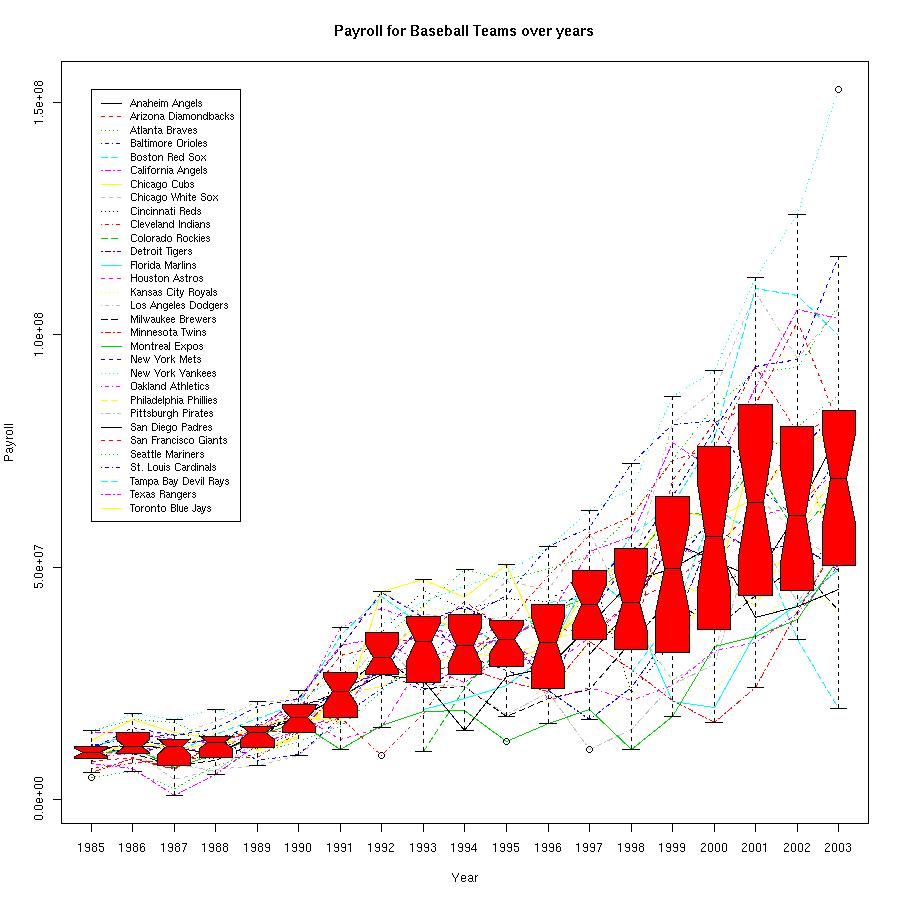
\includegraphics[width=5.5in]{RDBMS/images/PayrollYear.jpg}
 \caption{Time series plot for payroll with a boxplot for each year showing the distribution of the total payrolls for the collection of teams.}
\label{fig:payrollYear}
\end{figure} 
\end{center}

\begin{verbatim}
boxplot(Payroll ~ Year, data = d,at = 1985:2003, add = TRUE, 
        col="red", lwd=2, notch = TRUE)
plot(0, xlim = range(d[,"Year"]), ylim = range(d[,"Payroll"]), 
     type = "n", ..., xlab = xlab, ylab = ylab)

sapply(1:length(dd), function(i) {
        lines(dd[[i]][,"Year"], dd[[i]][,"Payroll"], col = i, lty = i)
        TRUE
        })

legend(min(d[,"Year"]), max(d[,"Payroll"]), names(dd), 
       col = 1:length(dd), lty = 1:length(dd), cex = .90)
\end{verbatim}

\begin{center}
\begin{figure}
 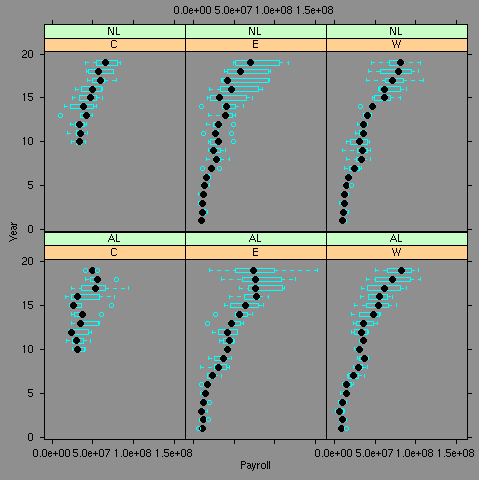
\includegraphics[width=5.5in]{RDBMS/images/PayrollPlotBW.png}
 \caption{A trellis/lattice-based boxplot of payroll versus year for each division with each of the two leagues (American and National)}
\label{fig:payrollYear}
\end{figure}
\end{center}

\begin{verbatim}
bwplot(Year ~ Payroll |  Division * League , 
       data = d, allow.multiple = TRUE)
\end{verbatim}

Augment the SQL statment above to include the following team
statistics for each season: the number of games in the season, the
number games won in a season, the information as to whether the
team won the division, wild card, league, or world series. To do
this you will need to join the table with the salaries with the
team table.

Use the xyplot in the lattice plot to explore the relationship
between payroll and performance. To do this, control for inflation
by cutting the data into six groups according to 3 year intervals,
and lay out six plots for these intervals. Construct a factor that
indicates whether the team won their division (or wild card),
league, or world series. The options are: no title, won division
or wild card but not league, won league but not the world series,
or won the world series.


\section{SQL for Statisticians}\label{dbms:sect:Smarties} 

Interfaces between statistical software and relational databases  
offer the opportunity to mix statistical analysis with
structured queries in flexible ways.
In fact, the flexibility poses the problem of determining 
where to do which computations: in SQL, in R, or split between
the two.
The choice depends on several issues, including
the available functionality in each environment,
the efficiency of the functionality in these environments, 
and the size of the data to be processed.

In this section we consider three examples: finding 
the three largest values of an attribute,
taking a random sample of tuples, and computing summary statistics
on grouped data. For each example, we present multiple solutions and
discuss the pros and cons of approach. 
We will use the RMySQL package to communicate in R with 
the database. 

\subsection{Ranking tuples}
Suppose we are interested in finding the the three highest 
salaries for baseball players in 2003.
The salary table in the baseball database is not very large.
We could easily pull the entire table into R 
and do all of the computations there.
\begin{verbatim}
sals = dbReadTable(con, "Salaries", row.names="playerID")
sort( unique( sals[sals$yearID == 2003,]$salary), 
      decreasing = TRUE)[1:3]
\end{verbatim}

Alternatively, the work can be done in SQL. As noted earlier,
the LIMIT clause can produce unreliable results when used with the
ORDER BY because of the order of operations, i.e. the limit is applied
before the tuples are ordered.  
The following SQL statement yields an ordered list of the distinct
values for salary:
\begin{verbatim}
orderSalary = dbGetQuery( con, 
     "SELECT DISTINCT Salary FROM Salaries 
        WHERE yearID = 2003 ORDER BY Salary DESC;" )
\end{verbatim}
Notice that we have pulled over all distinct salary values. 
An improvement on this approach uses dbSendQuery to avoid bringing
all of the sorted salary values into R.
\begin{verbatim}
res = dbSendQuery( con, 
      "SELECT DISTINCT Salary FROM Salaries 
         WHERE yearID = 2003 ORDER BY Salary DESC;")
topSalary = fetch( res, n = 3 ) 
dbClearResult( res ) 
\end{verbatim}

Celko provides an SQL solution to this problem that avoids sorting 
the salaries.
To understand it, it helps to think in terms of a sequence of nested subsets.
The goal is to assign a ranking to a subset of the table.
This subset contains the rows that have an equal
or higher value than the value that we are looking at.
Below, the Salary table with alias S1 provides the copy of the tuples 
to examine and the alias S2 provides the set of boundary values.
\begin{verbatim}
SELECT S1.Salary, 
     (SELECT COUNT(Salary) FROM Salaries AS S2
        WHERE S2.Salary > S1.Salary) AS Rank
  FROM Salaries AS S1;
\end{verbatim}

Another approach pulls the data into R in batches.
It finds the highest three salaries in a batch, and compares 
these salaries with the highest three in the previous batch. 
It is useful in the situation where we have more data than 
can easily fit in our R session or that can be sorted
in its entirety.
\begin{verbatim}
totCount = dbGetQuery( con, 
     "SELECT COUNT(*) FROM Salaries 
        WHERE yearID = 2003;")
res = dbSendQuery( con, 
     "SELECT Salary FROM Salaries 
        WHERE yearID = 2003;")

blockSize = 200
topSalary = NULL

for (i in ceiling(totCount[[1]]/blockSize)) {
    topSalary = sort( 
         unique( c(topSalary, fetch( res, n = blockSize)[[1]])),
         decreasing = TRUE )[1:3]
}

dbHasCompleted(res)
\end{verbatim}
Note that the last batch may be smaller than the blocksize
but the fetch will not give us an error when we ask for
more records than are left.
Note also that if our goal were to compute a median, 
this approach would not work.

If the ultimate goal is to find the players 
that correspond to the three highest salaries, we return to the 
database, and query the Salary table for the playerIDs that correspond
to the highest salaries (there may be more than three).
One way to do this, is to paste together a query that contains
the three salary values,
\begin{verbatim}
charSalary = paste( orderSalary[[1]][1:3], collapse = ", " )
cmd = paste( "SELECT playerID FROM Salaries WHERE yearID = 2003 
                 AND Salary IN (", charSalary, ") ;", sep = "" )
dbGetQuery( con, cmd )
\end{verbatim}

\subsection{Random sampling}
At times we want to work with a representative subset of the data.
For example, a graphic based on a subset may offer a clearer picture of
underlying patterns than one based on the entire data. 
SQL does not contain a pseudo random-number generator, and as shown
in Section~\ref{rng:sect:algorithm}, programming one from scratch
is not a good idea if you need a good random sampling procedure.
Sampling is a fundamental aspect of statistics, and so
well-tested pseudo random-number generators are a part of most 
statistical software. 
It appears that the selection process will need to be done in R. 
Even so there are many possible approaches to take.

Suppose we wish to take a sample of connections from the TCPConnections
table in the Network database.
Most simply, we can pull the key to the table across into R,
sample from it, and construct a query based on this sample
to get the corresponding records.

\begin{verbatim}
ConnID = dbGetQuery( con, "SELECT conn FROM TCPConnections;" )

sampleID = sample( ConnID$conn, 200)

sampleCharID = paste( sampleID, collapse = ", ")

sampleData =  dbGetQuery( con, 
                paste( "SELECT * FROM TCPConnections 
                        WHERE conn IN(", sampleCharID, " );", 
                        sep = "" ) )
\end{verbatim}

Two potential drawbacks to this approach arise: 
the entire index column is retrieved in order to sample from it,
and the set of sampled indices may get very long.  
We provide alternatives that address each of these possible problems.
First, if the key is an auto-increment type then it will have
values 1 through COUNT(*), and we can use this knowledge to 
generate the sample indices without having to pull the key attribute
into R.
\begin{verbatim}
totCount = dbGetQuery( con, "SELECT COUNT(*) 
                             FROM TCPConnections;" )
sampleID = sample( totCount, 2000)
\end{verbatim}
If the key is not such an index, one can be created with a temporary
table that consists of two attributes, the auto-increment index
and the original key attribute. 

\begin{verbatim}
 IDMatrix = matrix(sample(totCount, 2000), nrow = 10 )
 sampleData = apply( sampleMatrix, 1, function(x) 
               { 
                 charID = paste( x, collapse = " ," )
                 monte = dbGetQuery( con, paste( "SELECT * 
                         FROM TCPConnections 
                         WHERE conn IN (", charID, " );", sep = "" ))
                 summary(monte) 
               }
             )
\end{verbatim}

To address the second problem, we can reduce the size of the list of
indices to appear in the sample, which need to be in the IN clause 
of the SELECT query by pulling the sampled tuples across in batches.
This would be accomplished similarly to the approach shown in
the previous example.


\subsection{Summary statistics for grouped data}
Working with random samples of rows from a table is one
way to reduce the size of the data for analysis.
Another way is to aggregate like tuples.
In the study of network connections, we want to examine
the behavior of the connections over time for different ports. 
Rather than examine individual connections, attributes for
connections in the same time interval could be summarized 
and studied.  To make this concrete, we could examine 
the 0.25, 0.5, 0.75 quartiles and the maximum total packets
sent for connections to port 20 in 15 minute time intervals.
The code in Figure~\ref{dbms:fig:TCPbundle}
is one such approach.
The observed time period March 1, 1999 to April 8, 1999 is
cut into 15 minute intervals.
The data are ordered according to port and the time the 
connection was made to that port and placed in a temporary table.
This table holds only those attributes (and ports) of interest.
Records are fetched into R in blocks of 30,000 in port/time sequence.
The time the connection was sent is converted into a 15-minute
interval factor, and once converted, the tapply function does 
the work of finding the summary statistics on all connections in 
each 15-minute interval. 
These summary statistics are then appended to those computed 
so far, and another batch of records are fetched.
Note that one time interval will be split across two consecutive
batches of records. This incomplete interval needs to be saved
from one fetch to the next. We ignore that aspect of the
problem here.

\begin{figure}

\begin{verbatim}
# Initialize the date variables for pooling the data
  mintime = ISOdatetime(1999, 3, 1, 5, 0, 0)
  maxtime = ISOdatetime(1999, 4, 8, 3, 0, 0)
  timebreaks = seq.POSIXt(mintime, maxtime, by = "15 mins")

# Select the ports to examine
  Ports = c(20, 21, 22, 23, 25, 37, 79, 80, 113)

# Use SQL to create a temporary table that has the data sorted in
# port/time of first packet and that has only the variables of interest.
  dbGetQuery(con,"CREATE TEMPORARY TABLE short SELECT
     least(port_a,port_b) as port, 
     first_packet as timeSent, 
     (total_packets_a2b+total_packets_b2a) as totPackets 
     FROM TCPConnections order by port, timeSent ;")

# This function pulls data in blocks from the temporary table.  
# The data are then aggregated into 15 minute time intervals.
# Summary statistics such as the total number of connections,
# and the quartiles of total packets sent are computed for each interval.

processBlk = function (ports = Ports, inc = 40000)
{
    portstats = vector(mode = "list", length = length( ports ) )

    for (i in 1:length(ports)) {
        cmd = paste("SELECT * FROM short WHERE port IN (",ports[i],")  ;")
        cmd2 = paste("SELECT COUNT(*) FROM short WHERE port IN (",ports[i],") ;")
        recs = dbGetQuery(con,cmd2)
        res = dbSendQuery(con,cmd)
        
        n=inc
        while (n < recs + inc) {
            portData = fetch(res, inc)
            class(portData[["timeSent"]]) = c("POSIXt","POSIXct")
              tb = timebreaks[ min( portData[[ "timeSent" ]] ) <= timebreaks &
                     max( portData[[ "timeSent" ]] ) >= timebreaks ]
              timeFac = cut.POSIXt(portData[["timeSent"]],tb)

\end{verbatim}
\end{figure}

\begin{figure}
\begin{verbatim}

# Accumulate the summary stats
# The first statistic is the number of connections in the time interval

            numCon = tapply( portData[[ 3 ]], timeFac, length)
            notNAs = sapply(numCon, function(x) !is.na(x))
            rown = names( numCon )[ notNAs ]
            xx = matrix(( numCon [ notNAS ]), ncol = 1, byrow = TRUE)

            statQ = tapply( portData[[ 3 ]], timeFac, 
                     function(x) quantile( x, c(0.25, 0.5, 0.75, 1) ))

            xx = cbind(xx, matrix( unlist( statQ ), ncol = 2, byrow=TRUE))

            portstats[[ i ]] = rbind( portstats[[ i ]], 
                   as.data.frame(xx, row.names=rown))
            n = n+inc
         }
         dbClearResult(res)
  }
}
\end{verbatim}
\caption{describe the task}\label{dbms:fig:TCPbundle}
\end{figure}

%Do We want to show another way to do this?

%\subsection{Least Squares?}
%Do a least squares in batches? Updating ....

%Some calculation where numerical accuracy matters

\begin{comment}

\section{Managing and Designing your own Database}\label{dbms:sect:design}

As a statistician working on a project, you may face 
decisions on how to organize and manage the data in the project,
including whether or not to use a relational database 
management system.
The overhead in setting up a database is significant so there
need to be good reasons for choosing to use a database over
a project-specific organization of the data. 
In this section, we review some considerations to bear in mind 
when making this decision, and we discuss the basics of 
creating and designing databases. 


\subsection{Considerations}
A first consideration in the decision whether or not
to use a relational database is to determine who will be using the data.
If the only application using the data is your application, 
then organizing it in a form suitable for your needs 
may be the most efficient way to go and a database may be unnecessary. 
On the other hand, when several applications require access to
the data, each with a different set of requirements, then a centrally 
maintained database may be needed to guarantee data integrity.

A database management system enforces data integrity in a number of ways.
As seen already, checks can be placed on columns to ensure that the
data have the right type, have appropriate values, and are not NULL.  
The deletion of a row from one table can be automatically
reflected in other tables, or such changes can be forbidden in a 
particular table to maintain consistency across tables.
Further, transactions where multiple clients are updating a 
table simultaneously can be controlled to avoid data loss,
and these transactions can be ``rolled back" to restore the state of
a database before a user began his changes.

Another issue is security.  
Access to data can be controlled at the database, table, or column level. 
Use of the database may be restricted in scope and in privilege.
Scope restrictions control the host from which a user can connect to 
a database and and whether a password is required.
Restrictions on privileges control the types of commands or queries
that a user may perform, such as allowing a user to issue SELECT
statements, to create and delete tables, or to shutdown the server.

A relational database management system provides fast access to 
selected parts of large databases, and it provides powerful ways 
to summarize and tabulate data. So the size of your data should
be a factor in your considerations as well as the type of data that
need to be stored. 
If data are being collected from a variety of locations and analysis
of the data will be on-going throughout the data collection process
then having a system that supports the dynamic nature of this process
and that support applications for data entry could be real time saver.

The question of who will be maintaining the data also plays a role
in the decision whether or not to use a database. 
Clearly, setting up a database involves up-front costs.
However, personal database management systems are becoming widely 
available and no longer need a team of experts to set up and 
maintain.


\subsection{Setting up a database management system}

The database management system is a software application that 
does what its name implies, it manages databases. 
It runs a server as a daemon that listens for client 
requests for connections; 
it controls access to its databases, including
managing simultaneous users of the same database;
and  it performs administrative tasks such as logging activity
and managing resources.

MySQL is one such database management system. It is open source and
based on the SQL standard.  Detailed installation instructions appear
on the MySQL website, www.mysql.com, and in Butcher \cite{Butcher}.
You will need to decide which version (i.e. stable or Beta) to
download from the MySQL site to install and whether to install the
binary or the source.  These decisions depend on whether: you need a
stable production environment; your application requires features that
only appear in the Beta version; your system has an atypical
configuration; and you want special options in MySQL which would
require installation from source.

We outline the steps required to install MySQL from source on a Linux system.
In order to run, the MySQL server needs a Linux user and group which are both
called MySQL. We begin by creating these (as root), 
\begin{verbatim}
groupadd mysql
useradd mysql -g mysql
\end{verbatim}

After downloading the source, unzip and untar it into /usr/local/src. 
Then proceed to \executable{configure}, \executable{make}, and 
\verb+make install+ the application. 
To get started, you may want to configure with simple options such as
\begin{verbatim}
./configure --prefix=/usr/local/mysql
\end{verbatim}
The next step is to create a directory in which the data will
be stored. The script \executable{mysql\_install\_db} creates the directories 
and base files for managing the databases.
That is, the database management system uses a database to manage
its databases.
To set file permissions and system configurations 
MySQL provides some standard configurations that can be copied.
\begin{verbatim}
chown -R root /usr/local/mysql
chown -R mysql /usr/local/mysql/var
chgrp -R mysql /usr/local/mysql
cp support-files/my-medium.cnf /etc/my.cnf
\end{verbatim}

Now the server is ready to be started.
It runs a daemon called \executable{mysqld} that listens for requests 
for a connection to the database.
To start \executable{mysqld}, it is advisable to run the shell script
\executable{mysql\_safe} that will ensure that the server keeps running
if an error occurs.
\begin{verbatim}
/usr/local/mysql/bin/mysql_safe --user=mysql &
\end{verbatim}
If the server fails to start, the error messages should indicate
whether the problem is with file permissions or because the server is
already running or if there is some other error.
Once the server is running, the client program \executable{mysqladmin} 
administers the system, allowing you to shutdown or ping the server
and to set root password among other things.

\subsection{Setting up a database}
After installing the database management system, you can create 
a database.  Either the \executable{msyqladmin} program or SQL queries
can be used to create a database.
For example, to create the bank database, we can issue the 
following command at the Linux command line,

\begin{verbatim}
mysqladmin create BankDB -u nolan -p
\end{verbatim}
or we can invoke MySQL and then issue an SQL query as follows,
\begin{verbatim}
mysql -u nolan -p
CREATE DATABASE BankDB;
\end{verbatim}

Both of these statements create an empty database with no tables.
The next step is to add tables to the database. 
To do this, we must specify the attributes and their data types. 
The SQL queries below specify to use the BankDB database 
and to create the Customers table in that database.

\begin{verbatim}
USE BankDB;
CREATE TABLE Customers 
   (CustNo INT(4) NOT NULL, 
    Name CHAR(20), 
    Addr CHAR(30), 
    PRIMARY KEY (CustNo));
\end{verbatim}
In the table creation, we define the attributes and make 
the attribute CustNo the primary key.
Tables can be listed with SHOW TABLES; and attributes can
be listed via the DESCRIBE statement.

\subsubsection{Populating Tables}

Once a table is set up, we need to populate it with tuples. 
We can insert one tuple at a time with the INSERT statement. 
Alternatively, the LOAD DATA statement enables a text file 
containing data to be loaded in bulk into the database.
The \executable{mysqlimport} command (not an SQL query) can be 
used in a similar way. 
Below we show three versions of the INSERT statement.
The first provides an ordered list of values to be inserted
into a tuple, the second provides a list of attributes each
followed by their value, and the third provides a list of
attributes followed by a list of values in the same order as
the listed attributes.

\begin{verbatim}
INSERT INTO Customers VALUES (1,"Smith,J","101 Elm");
INSERT INTO Customers Addr = "101 Elm", CustNo = 2;
INSERT INTO Customers (CustNo, Addr) (3, "17 Spruce");
\end{verbatim}

\subsubsection{Consistency}\label{dbms:sect:consistency}
When we create multiple tables we typically need to connect a
record in one table to a record or records in another table.
In the bank example, the attribute CID in the Registration
table is a key to the customers in the Customer table.
For this reason, we call CID a foreign key.  
At the time a table is set up, we can place 
restrictions on changes that can be made to a key in a table 
and how changes in one table are to be reflected in another.
For example, in the query below, we set up the Accounts table
where AcctNo may not be set NULL and Branch may hold only two 
possible values (``City" and ``Suburb").
In addition, AcctNo serves as the primary key for the table,
and the attribute Branch references the Branch attribute in the 
Branches table. 
Changes to Branch in the Branches table have been constrained as
follows: 
when the value for Branch is changed in the Branches table, 
then the change will ``cascade" to the Accounts relation, 
i.e. it will change correspondingly, 
and when a tuple is deleted in the Branches table then the 
those tuples with the same value for Branch in the Accounts table 
will be set to NULL.

\begin{verbatim}
CREATE TABLE Accounts 
       (AcctNo INT(6) NOT NULL,
        Balance FLOAT(10,2), 
        Branch CHAR(8) CHECK (TYPE="City" or TYPE="Suburb"),
        PRIMARY KEY (AcctNo)
        FOREIGN KEY (Branch) REFERENCES Branches(Branch)
               ON UPDATE CASCADE ON DELETE SET NULL;
\end{verbatim}

Once a table has been created, the ALTER statement may be used to 
make changes to the table definition. Columns can be added, changed,
dropped, and renamed.  Keys can be added and tables themselves can
be renamed. Below is an example where the data type of an attribute
in the Branches table is modified.

\begin{verbatim}
ALTER TABLE Branches MODIFY Address CHAR(30);
\end{verbatim}

\subsubsection{Handling transactions and elimination of records}
The specifications in the declaration of a table helps maintain
integrity of the data in the table. For example, if an attribute
is specified as a primary key, then a tuple containing a
duplicate entry for the primary key can not be inserted into the
table.  Further, when the value of a primary key is changed in a
table, these changes are reflected in other tables provided the
specifications are given as shown in Section~\ref{dbms:sect:consistency}.
To change data that has already been entered into a table, 
we can update it as follows,

\begin{verbatim}
UPDATE Accounts SET AcctNo = 101 WHERE AcctNo = 201;
\end{verbatim}

At times we want to eliminate an entire database or table.
The DROP statement allows us to do this.
If we only need to remove a subset of tuples in a table then
we use the DELETE statement.

\begin{verbatim}
DELETE FROM Accounts WHERE AcctNo in (302, 201);
\end{verbatim}

\subsubsection{Access, Privileges, Security}
To allow users other than the one who set up the database to access 
the data, we need to GRANT privileges to them.
One common type of privilege to grant allows a user to only perform 
SELECT queries.
The following statement gives the user \SName{nolan} permission to 
issue SELECT queries
on all tables in the BankDB database when connected from the local host.

\begin{verbatim}
GRANT SELECT ON BankDB.* TO nolan@localhost;
\end{verbatim}

At the other extreme, a user may be given the privilege to perform
all types of queries on a database except for the GRANT. 
The following GRANT gives the nolan user all privileges, except GRANT,
on all tables in the BaseballDatabank database when connecting from any host 
provided that password npass is supplied. 

\begin{verbatim}
GRANT ALL ON BaseballDatabank.* TO nolan@"%" 
                 IDENTIFIED BY "npass";
\end{verbatim}

The MySQL database holds the grant table that control the 
privileges for the users of databases on the client.  
It is called \SQLName{mysql} and contains five tables that control 
privileges at five different levels: \SQLName{user, db, host, tables\_priv, 
and columns\_priv}.

Privileges can be ascertained from the 
\begin{verbatim} SHOW GRANTS FOR nolan@"%";\end{verbatim}
and they can be revoked with the REVOKE statement.
In order to connect to the database, the user must be present in the
\SQLName{user} table.
There privileges can be set for all databases on the server.
For example, a user may be given SELECT privileges on all databases.
If the SELECT privilege in not granted at this level,
when a user attempts to SELECT from a table in a particular database
then the \SQLName{db} table is checked to see if that privilege
is granted on that database.
Continuing in this way, if permissions are not given at the
database level, we proceed to the table level, which appears in
the \SQLName{tables\_priv}, and then on to the column or attribute level
permissions found in \SQLName{columns\_priv}.



\subsection{Designing Schema}
Database design is the process of deciding how to organize data 
into tables and records and how the tables will relate to each other.
The database should mirror the organization's data structure and process 
transactions efficiently.

We consider an example from a hypothetical survey of health and dietary 
habits of teenage girls. 
To develop a schema for the survey data, we first consider the 
survey process, and identify where definable events occur, 
e.g. the initial survey, visits to the doctor, etc.  
The survey will be ongoing over several years, where high school 
students are chosen to participate in the survey according to a two-stage 
sampling approach. In the first stage, a set of high schools are chosen at 
random, then in the second stage a random sample of students are selected
from each high school.  
This sampling occurs in waves over the course of several years.
The students in each wave complete an introductory
questionnaire, keep track of the food they eat each day in diaries 
over several months, and have scheduled checkups with their doctors.
In addition, teachers fill out questionnaires giving their views on
the participating students. 

From this brief description of the survey, two entities immediately
surface: the student and the high school.
It seems natural to have a table containing information on the 
students surveyed.
This may contain the student's name, address, and high school, 
demographic data such as age, grade-level, race, and family income, 
the food diary, lab tests from the doctor visits, and 
teacher interviews about the students.
The high school entity might simply contain the high school name and address.

\begin{figure}
\begin{verbatim}
Smith,J  101 Elm        Jefferson High 
 Day 1: 1300    Day 2: 1900     Day 3: 2100 ... Day 17: 1900  
 Visit 1: 29.7  Visit 2: 29.8   
 Dr. Reed, X Medical Group      
 Ms Martin      7.5   

Brown,D  12 Oak         Jefferson High 
 Day 1: 1100    Day 2: 2100     Day 3: 2300 ... Day 15: 1700  
 Visit 1: 18.1  Visit 2: 18.8   
 Dr. Reed, X Medical Group      
 Ms Martin: 5.5  Mr Green: 4.8   

Ritter,L         2015 Main              Highland High 
 Day 1: 1900    Day 2: 2000     Day 3: 2100 ... Day 21: 1400  
 Visit 1: 24.1  Visit 2: 23.8   Visit 3: 23.5   
 Dr. Eisen, Y Family Practice   
 Ms Max: 9  

\end{verbatim}
\caption{Data in a ragged array from a hypothetical sample survey. 
Notice that the number of calories consumed were recorded for a varying number
of days for each participant, and the number of doctor visits and teacher
reviews is not constant across participants.}\label{dbms:fig:CTragged}
\end{figure}

An oversimplified version of the student data appears in 
Figure~\ref{dbms:fig:CTragged}. 
The data contain information on three hypothetical students in the survey.
There we see the student's daily calorie consumption,
Body Mass Index recorded at doctor's visit, the doctor's name and clinic, 
and the teacher's name and numeric evaluation.
Notice that these data form ragged arrays. That is, students do not record
their calorie intake for the same number of days, they do not all visit the
doctor the same number of times, and they do not all have the same number of 
teacher evaluations. A database table must be rectangular, i.e. it must
have the same number of columns in each row. We do not have this in our 
survey data.  
This problem can be addressed by including in each student's record
say 30 daily diet columns, six doctor visits columns, and three teacher 
evaluation columns, where 30, six, and three are chosen as upper limits
on the number of days, doctor visits, and teacher evaluations, respectively. 
Several drawback to this approach immediately surface: 
student records would typically have many empty cells for most do not 
use the maximum allowed for these activities, 
but a student might unexpectedly exceed the maximum number of columns allowed.
A better approach would be to recognize that these ragged arrays
each represent an entity, namely a daily diet, a visit to the doctor, 
and a teacher's evaluation. 
Therefore each deserves its own table. 

Take for example the doctor visits.  A doctor-visit table
could be designed as in Figure~\ref{dbms:fig:visits}, 
where the data for the doctor's visits has been split off from the 
student record in Figure~\ref{dbms:fig:CTragged} into a separate table.
Note however that two problems have arisen, the doctor's name is 
redundant as it now appears in each visit tuple and the connection between
the student and the visits to the doctor has been lost.
We remedy the second problem by adding to the visit table an 
attribute that identifies the student. 
Rather than use the student's name, it is more suitable to
add a student identification number to the table because 
names and other personal data for participants in surveys 
are often kept confidential.
Instead of putting this confidential information in many tables,
it makes sense to keep it in one table, to identify individuals by an
uninformative identification number, and to place security constraints
on the single table with names. 

\begin{figure}
Doctor Visit \\
\begin{tabular}{llll}
Date & Lab results & Doctor & Clinic\\
1& 19.7  & Dr. Reed & X Medical Group\\  
2& 19.8 &  Dr. Reed  & X Medical Group\\
1& 18.1 &  Dr. Reed & X Medical Group\\ 
2& 18.8 &  Dr. Reed & X Medical Group\\ 
1& 21.1 &  Dr. Eisen & Y Family Practice\\
2& 20.8 &  Dr. Eisen & Y  Family Practice\\
3& 20.5 &  Dr. Eisen & Y Family Practice\\
\end{tabular}
\caption{The data for the doctor's visits has been split off into 
a separate table. 
Note however that two problems arise, the doctor's name is redundant
appearing in each visit and the connection between 
the student and the visits to the doctor has been lost.}\label{dbms:fig:visits}
\end{figure}

That leaves the problem of redundancy of the doctor's name and 
clinic in the Visits table.
One doctor oversees many visits for a single student so it makes more 
sense to identify the doctor in the student table. 
This removes the redundancy from the visit table, 
but if we include the doctor's name and location in the student file, 
we still have redundant information. 
A doctor sees many students, and the doctor's clinic is information
about the doctor, not about the student. 
That is, we have identified another entity, the doctor.
A doctor table would contain, a doctor's identification number,
name, and clinic. The doctor's identification number would 
then appear in the student table to connect her with the students she treats.
The schema for the revised Visits table, the new Doctor table, 
and the Student table all appear in Figure~\ref{dbms:fig:schema}.
We see there that we also need a diary table and an evaluation table to hold 
the data in the diary entries and the teacher evaluations.

\begin{figure}

Students\\
\begin{tabular}{|lll|}
\hline
StudentId &  &  \\
Name &  &  \\
Address &  & \\
DoctorID &  & \\
HighSchool &  & \\
\hline
Diary & 0 & N\\
Visits & 0 & N\\
Evaluations & 0 & N\\
\hline
\end{tabular}

\medskip

Diary Entries\\
\begin{tabular}{|lll|}
\hline
StudentId &  &  \\
DayId &  & \\
Calories &  & \\
\hline 
Students & 1 & 1 \\
\hline
\end{tabular}

\medskip

Evaluations \\
\begin{tabular}{|lll|}
\hline
StudentId &  & \\
TeacherId &  &  \\
Score &  &  \\
\hline
Students & 1 & 1\\
Teachers & 1 & 1\\
\hline
\end{tabular}

\medskip

Visits \\
\begin{tabular}{|lll|}
\hline
StudentId &  &  \\
VisitId &  & \\
BMI &  & \\
\hline 
Students & 1 & 1 \\
\hline
\end{tabular}

\medskip

Doctors \\
\begin{tabular}{|lll|}
\hline
DoctorId &  & \\
Name &  & \\
Clinic &  &  \\
\hline
Students & 1 & N\\
\hline
\end{tabular}

\medskip

Teachers \\
\begin{tabular}{|lll|}
\hline
TeacherId &  &  \\
HighSchool &  & \\
Name &  & \\
\hline
Evaluations & 0 & N\\
HighSchool & 1 & N\\
\hline
\end{tabular}

\medskip

HighSchool \\
\begin{tabular}{|lll|}
\hline
Name &  &  \\
Address &  & \\
\hline
Teachers & 1 & N\\
Students & 1 & N\\
\hline
\end{tabular}

\caption{In this figure there is one ``table" for each entity, and in this 
table the attributes are listed.
Also connections to other entities are displayed. 
For example, within the Patient entity, we see that one patient may
have no tuples in the Visit table, one tuple, or many tuples.}\label{dbms:fig:schema}

\end{figure}

Finally, consider the relationship between teachers and high schools.
This relation is many-to-many meaning that one high school has
many teachers and on teacher may teach in many high schools.
Thus a teacher-high school entity, 
where each tuple is uniquely identified by the teacher-high school
pair, is required to handle this many-to-many relation. 
These types of tables are sometimes called linking tables.
It appears in Figure~\ref{dbms:fig:schema}. 

Figure~\ref{dbms:fig:schema} lays out the schema for the
database, where each entity is identified along with its attributes 
and its relations to the other entities.
The pair of numbers that follows the related tables 
specifies bounds on the number of tuples in these tables that 
a tuple in the given table may have.
For example, in the Student entity, we see that one student may
have between 0 and many tuples in the Visit table, whereas 
a visit instance in the Visits relation must have one and only one
student entity. 
Thus we identify the many to one relation between students and visits.

By describing the survey process, removing ragged arrays and redundancies
of the two types we encountered, we have arrived at a reasonably well designed
schema that is in what is called third normal form.  
Normal forms are essential for efficient data processing. 
See Rolland \cite{Rolland} for more details on normal forms.
                                                                      

\section{Alternatives to Databases}

Relational database tables are neither spreadsheets nor files.  In a
spreadsheet, cells in a workbook can contain instructions rather than
data; there is no conceptual difference between a row and a column,
i.e. they can be transposed; and the spreadsheet can be navigated with
a cursor.

Factors to consider: setup, maintenance, scale

As for flat files, the fields in a file are defined in the program,
not in the file itself; files are processed one line at a time,
whereas in a relational database we connect to a a suite of tables and
work with the table as a whole entity; empty tables are still valid
tables for performing operations, while an empty file typically
requires special treatment, e.g. an EOF flag to handle clean up.

\cite{Celko}
%[[Reference SQL for Smarties]]


Flat files, file systems, XML, Object databases, etc.



\putbib[RDBMS/dbms]
%\cite{Celko}
\end{bibunit}
\end{comment}

\section{Exercises}

The following exercises all use the baseball databank.

\begin{enumerate}
\item How many people are included in the databases?
\item Are all of these players? How many are players? how many are managers? and how many are both?
\item     What is the earliest season recorded in this database? and the most recent?
\item  What college produced the largest number of major league baseball players? Is there a geographical trend? How many colleges are there in total? And how many players didn't go to college at all?
\item  Can we tell who won the "World" series in a given year?
\item  Who lost the "World" series in each year?
\item Look at the relationship between the number of games won in a season and winning the world series? And similarly relate these to payroll.
\item  Plot the payrolls over years for the different teams. What plot types are good for showing this data? Contrast different graphical techniques. Information for inflation rates from 1986 to the present is available in the database inflation and in the relation AnnualRates. You might consider using this to adjust/control the dollar amounts for inflation.
      Superimpose the payroll of the two teams that made it to the "World Series" on this plot. Is there a relationship? How about for the teams that made it into the playoffs in a year?
\item Show the distributions of the payrolls over years. We can think of a boxplot for each year for this. Again, we can superimpose additional attributes and even lines connecting the different statistics for particular teams if they are not very noisy.
\item  Look at the payrolls for the teams that are in the same leagues? and then in the same divisions? Are there any interesting characteristics?
\item Is the payroll related to the age of the players? One might expect an old team to be paying veteran players a lot near the end of their careers. Teams with a large number of older players would therefore have a large payroll. Is there any evidence supporting this?
\item Look at the distribution of salaries of individual players over time for different teams.
\item Look at players and see whether the distribution of home runs has increased over the years?
\item Are Hall of Fame players, in general, inducted because of rare, excellent performances or years or are they rewarded for consistency over years?
\item Are certain baseball parks better for hitting Home Runs? Can we tell from this data? Can we make inferences about this question?
\item Do teams with a few good players and many mediocre players tend to do better than a team made up of more homogeneous talent?
\item Look at the distribution of how well batters do. Does this vary over the years? Do the same players excel each year? Is there a clustering? a bi-modal distribution?
\item Do pitchers get better with age? Is there an improvement and then a fall off in performance? And is this related to how old they are? the number of years they have been pitching? which league they are in and the designated hitter rule? Do we have information about each of these factors and how can we combine them to present information about the general question?
\end{enumerate} 

%\bibliographystyle{plain}
%\bibliography{RDBMS/dbms}
 

\chapter{Basics of XML}
\section{The structure of XML}
\section{Parsing XML}
 \subsection{xmlParse}
 \subsection{XPath}
 \subsection{htmlParse}
 \subsection{xmlEventParse}
 SAX event parsing
 \subsection{xmlTreeParse}
 R-based objects

\section{Generating XML within R}
 \subsection{HTML}

\chapter{Web Services}
 \section{HTML Forms}
 \section{REST}
   \subsection{GET and parameters}
 \section{RCurl}
   \subsection{Controlling the HTTP request}
 \section{SSOAP}
   \subsection{.SOAP}
   \subsection{WSDL}



\chapter{Efficient Code}
This chapter is concerned with making code run quicker or with less
memory.  We start by measuring the time a function or piece of code
takes to run as a function of the size of the inputs.  This introduces
the notion of empirical algorithmic complexity.

We then discuss how to write efficient code, i.e. code
that runs quickly and does not use excessive memory.  We present some
general rules to keep in mind when writing R code, or indeed code in
most languages.  We illustrate the effects of these guidelines on some
relatively simple examples to show how much improvement we obtain. 

We then move on to general tools for identifying which code

 \section{system.time, gc, --min-vsize}
 \section{Pre-allocating results rather than concatenation}
 \section{Avoiding Recalculation}
   Here we talk about the obvious idea of avoiding recomputing
   expressions that we don't have to. This arises often when we 
   try to 
 \section{Profiling}
   \Rfunc{Rprof}
 \section{Memory Profiling}
   \Rfunc{tracemem}

\section{Compiled Code}
 The next step in making code run more quickly is to use a faster
 programming language.

 \subsection{The Anatomy of Compiled Code}
  Compilation, linking, loading
  dyn.load
  nm, ldd/otool, %\env{(DY)LD\_LIBRARY\_PATH}
  \subsubsection{Why is C code faster than R code?}
  \subsection{.C}
  \subsection{.Call}

  \subsection{Interfacing to C++}  
     extern and name mangling
   \subsubsection{Rcpp}
   \subsubsection{Implementing and Extending C++ classes with R functions}
  \subsection{Using dyncall}
  \subsection{Automating the Process: GCC Translation Unit}
  \subsection{SWIG}
  \subsection{Type libraries on Windows}


 \section{Basics of High Performance Computing}
   (This might be a separate chapter)





\chapter{Software Tools}

\section{Version Control}
 make (ant), version control (svn or git)

\section{Literate programming}

\section{R Tools for working with source}
 (e.g. ptoc, codetools, CodeDepends)

\section{}
 patch \& diff

\section{shell scripting}

  test

\section{Configuration and Portability}

 autoconf, configuration and portable code.


 sed, (g)awk

 find

 cron jobs

\section{File Permissions}
 file permissions


\chapter{Distributing Software}
  \section{R Packages}
   \subsection{Basics}
   \subsection{Name Spaces}

 \section{Installing 3rd party code}
   without having adminstration privileges

\chapter{Dynamic Documents and Reproducible Research}
%Sweave, XDynDocs, RWordDynDoc

Here we talk about the concept of dynamic documents 
in which code is inserted into the document where the results
are supposed to be. Then we process the document and 
evaluate the code and insert the results of the computations.
\section{Sweave}
\section{XDynDocs}
\section{odfWeave}
\section{RWordDoc}


\chapter{Object Oriented Programming}
In this chapter we discuss the basic ideas and merits of
object-oriented programming.  The idea is to introduce method
dispatch, polymorphism, structured type defintions.
We will go through several reasonably involved examples/case-studies
which illustrate how to think about designing and programming S3 and
S4 classes.

\section{S3 Classes and Methods}
 This is the simple and marginally old-fashioned approach to 
 
   
 \section{S4 Classes and Methods}
 Here we discuss the S4 class and method mechanism.


 \section{Combinging S3 and S4}
 In some cases, we will have S3 classes and we won't want to update
  them to S4 classes.  However, we will want to use some of these classes
  with S4 methods.  So we will have to understand how these interact.


\chapter{Graphical User Interfaces}
\textbf{Much of this will come from our wxWidgets paper.
However, we might target Qt.}

  \section{Toolkits: Gtk, wxWidgets, Qt, Tk, gWidgets}
   We do not focus on Tk, but rather the other three toolkits and
   their relative merits and similarities.
  \section{Widgets}
    We discuss the creation of widgets in the different toolkits.
  \section{Callbacks}
    We present the ideas of signals, events and event handler functions.
   \subsection{Closures/Lexical Scoping}
     Here  we talk about how we can define a collection of functions
     that  share a set of variables that are unique to a particular
     instance of a GUI. 
     This is the notion of scoping based on closures or lexical scoping.
  
  \section{GUI Designers}
     Using GUI applications to create GUIs interactively.
     libglade, wx's GUI designer
  \section{Mozilla}

\chapter{Inter-system interfaces}
 \section{General Philosophy}
Here we discuss the general idea of inter-system interfaces.
This is the idea that the programmer in one language can call
functions written in another as if they were  native to the programmer's own
language.  The idea is very simple but frequently not used. 


 \section{RSPython/Rpy}
 This illustrates how we can call Python functionality and classes
 from R and R functionality from R.  We work through different case
 studies/examples that illustrate the utlity of Python as a scientific
 programming language in combination with R.
 \section{RSPerl}
  We look at how we can can interact with Perl from R and vice-versa.
  Again, there are lots of examples such as processing email messages.
 \section{rJava/RSJava}
  There are two R-Java  bridges. These allow R programmers to
  interface with Java classes and methods in different  manners.
  Similarly, Java programmers can use R functionality.

 \section{DCOM}
 CORBA and DCOM are what are called middle-ware.  They act as brokers
 between applications to provide ``remote procedure invocation''.  We
 show how we can use R as a DCOM client using either RDCOMClient or
 rcom.  We also show how we can export a collection of R functions to
 implement an server object via RDCOMServer.  We use the combination
 of RDCOMServer and RDCOMClient to implement DCOM event handlers (via
 RDCOMEvents).

%\part{Visualization}

%\chapter{Advanced Graphics: Grid}


\chapter{Advanced Visualization: Interactive, Annotated Graphics}

\section{Low-level graphics: grid}

\section{SVG}
\section{Flash MXML}
\section{KML}

\section{rgl}


\end{document}
